
\documentclass[a4paper, 12pt]{article}
\usepackage[top=3cm, bottom=3cm, left = 2cm, right = 2cm]{geometry} 
\geometry{a4paper} 
\usepackage[utf8]{inputenc}
\usepackage{textcomp}
\
sepackage{graphicx} 
\usepackage{amsmath,amssymb}  
\usepackage{bm}  
\usepackage[pdftex,bookmarks,colorlinks,breaklinks]{hyperref}  
\hypersetup{linkcolor=black,citecolor=black,filecolor=black,urlcolor=black} % black links, for printed output
\usepackage{memhfixc} 
\usepackage{pdfsync}  
\usepackage{fancyhdr}
\usepackage{enumitem}
\usepackage{color,soul}
\usepackage{cite}
\usepackage{txfonts}
\usepackage{setspace}
\usepackage{siunitx}
\usepackage{lipsum}
\usepackage{natbib}
\usepackage{cancel}
\usepackage{eucal}
\usepackage{physics}
\pagestyle{fancy}
\newcommand{\tn}[1]{\textnormal{#1}}
\graphicspath{{./images}}
\doublespacing

\title{Utrecht University\\
        \large Cosmology\\}
\author{Yamamoto Sho}


%\date{}
\begin{document}
\maketitle
\tableofcontents

\section{Midterm recap}
\label{sec:Midterm recap}
  
In this section we review the most important concepts for the midterm. 

\subsection{Evolution equations}%
  \label{sub:{Evolution equations}
  

The Friedmann equations are, 
\begin{align}
  \label{friedmann equations}
    H^2(t) &= \frac{8\piG}{3} \rho  \\ 
    \frac{\ddot{a}}{a} &= - \frac{4\piG}{3}(\rho + 3P) 
\end{align}, where often we take \( P = \omega \rho \). 
We also couple these with the conservation of energy, 
\begin{align}
  \label{consevation of energy}
  a^{-3} \frac{\dd[]{(\rho a^{3} )}}{\dd[]{t}} = - 3
  H P 
\end{align}

\subsection{Components of the Universe}%
  \label{sub:Components of the Universe}

  \begin{enumerate}
    \item[\circ] matter: \( \rho_m  = \rho_{m, 0} a^{-3}  \) \\ 
    \item[\circ]  radiation: \rho_r = \rho_{r, 0} a^{-4} \\ 
    \item[\circ]  \rho_{\Lambda} = \frac{\Lambda}{ 8 \pi G } = -
    P_{\Lambda}
  \end{enumerate}
And the general expression for a perfect fluid is \( P = \omega \rho \), and
in the CPL parametrisation for DE: \( \omega(a) = \omega_0 +
\omega_{a}(1-a) \)

\subsection{Distances in the Universe}%
  \label{sub:Distances in the Universe}
  There are numerous distance indications for cosmology, the primary
  ones are, 
  \begin{enumerate}
    \item[\circ] Comoving distance: 
    \begin{align}
      \label{comoving distance}
      \chi(a) = \int_{a(t)}^{1}
      \frac{\dd[]{a^{\prime}}}{a^{\prime 2} H(a^{\prime}) },
      \hspace{0.5cm}\mathrm{ or }\hspace{0.5cm} \chi(t) =
      \int_{t}^{t_0} \frac{\dd[]{t^{\prime}}}{a(t^{\prime})}, 
    \end{align}
    \item[\circ] Redshift:
    \begin{align}
      \label{redshift}
      1 + z \equiv \frac{\lambda_{\mathrm{obs}}}{\lambda_{e}} =
      \frac{1}{a(t_e)}
    \end{align}
    \item[\circ] Luminosity distance: 
    \begin{align}
      \label{luminosity distance}
      F \equiv \frac{L}{4 \pi d_{L}^{2}(z)} \hspace{0.1cm}
      \mathrm{then} \hspace{0.5cm} d_{L}(z) = \chi(z) (1 + z)
    \end{align}
    \item[\circ] Angular diameter distance: 
    d_{A} \equiv \frac{L}{\delta \theta} \hspace{0.1cm}
    \mathrm{then} \hspace{0.5cm} d_{A}(z) = \frac{\chi(z)}{(1+z)}
  \end{enumerate}

  \subsection{Key concepts in thermal history}%
    \label{sub:Key concepts in thermal history}
    The three main key concepts in thermal history are 
    \begin{enumerate}
      \item[\circ] Redshift of equality \( \Omega_{m, 0}
      a_{\mathrm{eq}}^{-3} = \Omega_{\gamma, 0}
      a_{\mathrm{eq}}^{-4} \)
      \item[\circ] Energy density in relativistic species scales as
      \( \rho_r \propto a^{-4}  \)
    \end{enumerate}
    


\section{Thermal History}
  \subsection{Planck time}%
    \label{sub:Planck time}
     We define the Planck time as \( \lambda_B = \frac{h}{M_{P} c}, r_s
     = \frac{2GM_P}{c^2} \), with the Planck mass defined as \( M_p =
     \sqrt{ \frac{hc}{2G} } = 10^{19} \mathrm{GeV}  \), we can also
     define \( t_p = \frac{2GM_P}{c^3} ≈ 10^{-43}s \) (btw this is
     where we define GR and QM breaks down time after the big bang
     singularity).  



  \subsection{Interactions}
    To talk about interaction, we start by defining the cross section 
    \begin{align}
      \label{cross section}
      \Gamma = \frac{\nu}{l} = n \sigma \nu
    \end{align}
    and the relevant scale in the evolution of all matters in
    cosmology is namely comparing \( \Gamma^{-1}   \) and \( H^{-1}  \) 
    \begin{align}
      \label{relevant cross section scale in cosmology}
      \begin{cases} 
        &\Gamma^{-1} \sim t_{\Gamma} \ll t_{H} \sim  H^{-1} \implies
      \textnormal{ freeze out (or equilibrium) } \\ 
        &\Gamma^{-1} \sim t_{\Gamma} \gg t_{H} \sim  H^{-1} \implies
        \textnormal{ still in interaction. } \\
         &\Gamma^{-1} \sim t_{\Gamma} \sim t_{H} \sim  H^{-1}
         \implies \textnormal{ decouple from the thermal bath
         (particle soup). }
      \end{cases}   
          \end{align}
    Very intuitive so I won't comment here, yet this very comment is a
    comment, quite contradictory indeed.
    For particles that are leftover, i.e. after decoupling, we coined
    them as relic abundance over that matter. Also, one often use
    temperature (of photon) as a way to indicate decoupling of a certain
    species in the x-axis, as in a sense it indicates time flow in the
    early universe.

    \subsection{Effective DOFs}%
      \label{sub:{Effective DOFs}

     We now introduce degrees of freedom (dof) in the early
     cosmology picture (not really "early" but hey ho).  
     For \underline{coupled species} of same \( T_{\gamma} \) 

     \begin{align}
      \label{coupled species}
       \rho = \sum_{i} \rho_i = \sum_B \frac{\pi^2}{30} g_i T^4 +
       \sum_F \frac{\pi^2}{30} \frac{7}{8} g_i T^4 =
       \frac{\pi^2}{30} g_{\star}^{th} T^4
     \end{align}
     where, 
     \begin{align}
      \label{eff dof th}
       g_{\star}^{th} = \sum_B g_i + \sum_F \frac{7}{8} g_i
     \end{align}
    And for \underline{decoupled species}.
    \begin{align}
      \label{decoupled species}
       \rho = \sum_{i} \rho_i = \sum_B \frac{\pi^2}{30} g_i T^4_i +
       \sum_F \frac{\pi^2}{30} \frac{7}{8} g_i T^4_i =
       \frac{\pi^2}{30} g_{\star}^{dec} T^4
    \end{align}
    where, 
     \begin{align}
      \label{eff dof dec}
       g_{\star}^{dec} = \sum_B g_i \bigg(\frac{T_i}{T}\bigg)^4 + \sum_F
       \frac{7}{8} g_i \bigg(\frac{T_i}{T}\bigg)^4
     \end{align}

     \textbf{\underline{Comment:}} We can be fairly reckless about
     computing (\ref{eff dof th}), but not for (\ref{eff dof dec}). 
      
      

      \subsection{Temperature evolution}%
        \label{sub:Temperature evolution}
        When a system is in equilibrium, it remains at a fixed
        entropy, which asks for a good place to start the analysis
        of temperature evolution, the corresponding formula to
        start with is none other than the \textit{second law of
        thermodynamics}.

       \textbf{\underline{Comment:}} Just so we are on the same page,
       we are trying to obtain the entropy density \( s \) in our
       following calculation, which serves numerous use in this whole
       temperature analysis.

        \begin{align}
          \label{second law of thermodynmaics}
          T \mathrm{d}S = \mathrm{d}U + P \mathrm{d}V.
        \end{align}, where we can further define \( U = \rho V \),
        thus 
        \begin{align}
          \label{2nd law in different form}
          V \mathrm{d}\rho + \rho \mathrm{d}V = T \mathrm{d}S - P
          \mathrm{d}V
        \end{align} 
        
        We then apply the energy conservation equation: 
        \begin{align}
          \label{energy conservation equation}
          \frac{\mathrm{d}\rho}{\mathrm{d}t} = -3 H (\rho + P).
        \end{align}
        
        and that \( V \propto a^3 \), so we can turn H into V, 
        
        \textbf{Checkpoint 1:}
        \begin{align}
          \label{checkpoint 1}
          \frac{\mathrm{d}\rho}{\mathrm{d}t} = - \frac{1}{V}
          \frac{\mathrm{d}V}{\mathrm{d}t} (\rho + P)
        \end{align} 
      
        And now we finally substitute (\ref{second law of
        thermodynmaics}) into (\ref{checkpoint 1}) and
        differentiating it with respect to time: 
        \begin{align}
          \label{2.21}
          - \frac{\mathrm{d}V}{\mathrm{d}t} (\rho + P) + \rho
          \frac{\mathrm{d}V}{\mathrm{d}t} = T
          \frac{\mathrm{d}S}{\mathrm{d}t} - P
          \frac{\mathrm{d}V}{\mathrm{d}t}.
        \end{align}
        which implies, 
        \begin{align}
          \label{entropy stays}
          \frac{\mathrm{d}S}{\mathrm{d}t} = 0.
        \end{align}
    
        This means the universe we assume here is a closed system
        which conserves entropy. And for convienience we introudce
        the \underline{entropy density} \( s \equiv S/V \), and
        change of variables into (\ref{2.21}) and get. 

        \begin{align}
          \label{2.23}
          V \mathrm{d}\rho + \rho \mathrm{d}V = T(s \mathrm{d}V + V
          \mathrm{d}s) - P \mathrm{d}V. 
        \end{align}
        
        And rewriting further and also realizing the following
        \hl{important} discussion. 
        \subsubsection{Important remark on Extensive and
        Intensive properties of thermodynamics quatities}%
          \label{sub:Important remark on Extensive and
                Intensive properties of thermodynamics quatities}
      
        Rewriting and we get 
        \begin{align}
          \label{2.24}
          \mathrm{d} \rho + T \mathrm{d}s = (Ts - \rho - P)
          \frac{\mathrm{d}V}{V}.
        \end{align}
        
        And note that the density and the entropy density are
        intensive properties on the \textnormal{L.H.S.}, this
        means that they do not depend on the extent of the system,
        and in this case depends only on the temperature, so
        \textnormal{L.H.S.} \( \propto \mathrm{d}T \) and
        \textnormal{R.H.S.} \( \propto \mathrm{d}V \). So we get
        something like \( C_1 \mathrm{d}T + C_2 \mathrm{d}V = 0  \),
        and for this to conserve then both \( C_i = 0 \), which
        means we get, 
        \begin{align}
          \label{entropy density}
          s = \frac{\rho + P}{T}
        \end{align}

       \begin{align}
        \label{entropy constant}
         S = s(T) a^3 = \bigg[ \frac{\rho(T) + P(T)}{T} \bigg] a^3
         = \mathrm{constant}.
       \end{align} 

       where \( a \) is the scale factor.
      
      Now, we know that for radiation matter, \( \rho \propto T^4
      \implies s \propto T^3 \), then we can once again rewrite the
      entropy density as multiple coupled and decoupled species, 
      \begin{align}
        \label{entropy density in coupled decoupled}
        s(T) &= \sum_i \frac{2\pi^2}{45}( g_{\star,
        S}^{\mathrm{dec}}(T) + g_{\star, S}^{\mathrm{th}}(T) )T^3. 
      \end{align}
    
    Now for species that are coupled, we see that \( g_{\star,
    S}^{\mathrm{th}} = g_{\star}^{\mathrm{th}}. \) And that for
    decoupled species, again need to consider the temperature
    difference from radiation, becomes 
    \begin{align}
      \label{eof for decoupled}
      g_{\star, S}^{\mathrm{dec}} &=  \sum_{i = b} g_i \bigg(
      \frac{T_i}{T} \bigg)^3 + \frac{7}{8} \sum_{i = f} g_i \bigg(
      \frac{T_i}{T}\bigg)^3.
    \end{align}

    \subsection{Consequences of entropy conservation}%
      \label{sub:Consequences of entropy conservation}
      \begin{enumerate}
        \item[\circ] \textbf{Evolution of the temperature with the
        scale factor:} Since \( g_{\star, S}^{} T^3 a^3 =
        \mathrm{constant} \implies T \propto g_{\star, S}^{-1/3} a^{-1}
        \propto g_{\star, S}^{-1/3} (1+z)  \).
      , this is only valid as long as we are far from
      mass thresholds where creation and annihilation cease to be
      efficient.
      \item[\circ] \textbf{Time evolution of the temperature of the
      Universe: } In radiation-dominated Universe, the scale factor
      evolves as \( a \propto t^{1/2} \implies T \propto
      g_{\star, S}^{-1/3} t^{-1/2}   \).
      \end{enumerate}

      \subsection{Neutrino decoupling}%
        \label{sub:Neutrino decoupling}
        Neutrino decoupling plays a big role in the overall
        temperature of the Universe, in this regime, we have the weak
        interactions that keeps neutrinios in equilibrium with
        other species, namely: 
        \begin{align}
          \label{neutrino reactions}
          \nu_e + \bar{\nu}_e &\leftrightarrow e^- + e^+ \\ 
          e^- + \bar{\nu}_e &\leftrightarrow e^+ + \nu_e
        \end{align}
        At roughly \( T_{\mathrm{dec}} \approx 1 \mathrm{MeV} \),
        these interactions becomes inefficient to keep in
        equilibrium, and the decoupled neutrinos now preserve a
        Fermi-Dirac distribution and their number density dilutes with
        the expansion of the universe as, 
        \begin{align}
          \label{neutrino density}
          n_{\nu} \propto \int \dd[3]{p} \frac{1}{\mathrm{exp}
          \hspace{0.1cm} (p/T_{\nu}) + 1}. 
        \end{align}
        Note that we also know the momentum of radiation scales as
        \( p \propto a^{-1}  \), and make a change of variable on
        (\ref{neutrino density}) with \( q \equiv pa \) and we see
        that 
        \begin{align}
          \label{neutrino density in terms of q}
          n_{\nu} \propto a^{-3} \int \dd[3]{q}
          \frac{3}{\mathrm{exp} \hspace{0.1cm} (\frac{q}{a
          T_{\nu}}+1)}. 
        \end{align}, but we know that \( n_{\nu} \propto a^{-3}  \)
        to obey particle number conservation after decoupling, so \(
        T_{\nu} \propto a^{-1} \) to keep (\ref{neutrino density in
        terms of q}) true.

\subsection{Positron electron annihilation}%
  \label{sub:Positron electron annihilation}
  Now we move on to positron electron annihilation period, 
  The relevant reaction is (and the temperature \( T \approx m_e \)), 
  \begin{align}
    \label{Positron electron annihilation}
    e^- + e^+ \leftrightarrow \gamma + \gamma
  \end{align}
  Here we wish to calculate the ratio \( T_{\gamma, 0}/T_{\nu, 0} \), and
  our starting point is getting the entropy density \( s \), to do so we
  first compute the dof, which is simply \( g_{\star} = 2 + 7/8(2 + 2 +
  3 + 3) \), this is because we have the following particles present at
  that moment, 
  \begin{align}
    \label{ particles present in p e annihilation }
    e^-, e^+, \gamma, \nu_{e}, \bar{\nu}_e, \nu_{\tau},
    \bar{\nu}_{\tau}, \nu_{\mu}, \bar{\nu}_{\mu}
  \end{align}
  The entropy density is thus, 
  \begin{align}
    \label{entropy density at p e annihilation}
    s(a_1) = \frac{43\pi^2}{90} T_{1}^{3}.
  \end{align}
  And after annihilation, we have the following particles only, 
  \begin{align}
    \label{particles present after p e annihilation}
     \gamma, \nu_{e}, \bar{\nu}_e, \nu_{\tau},
    \bar{\nu}_{\tau}, \nu_{\mu}, \bar{\nu}_{\mu}.
  \end{align}
  Thus dof has been reduced to 2 for the photons and 6 for the neutrinos,
  but both at different temperatures, so that we have, 
  \begin{align}
    \label{entropy density after p e annihilation}
    s(a_2) &= \frac{2\pi^2}{45} \bigg( 2 T_{\gamma}^{3}(a_2) +
    \frac{7}{8} 6 T_{\nu}^{3} (a_2) \bigg).
  \end{align}
  Next, apply conservation of entropy, i.e. \( s(a_1) a_{1}^{3} = s(a_2)
  a_{2}^{3} \), and at the same time, we use \( a_1 (T_1 =
  T_{\gamma}) = a_2
  T_{\nu}(a_2) \)
  So putting everything together, we shall get, 
  \begin{align}
    \label{radiation neutrino ratio}
    \frac{T_{\gamma}(a_2)}{T_{\nu}(a_2)} = \bigg( \frac{11}{4}
    \bigg)^{1/3} 
  \end{align}
  And knowing CMB temperature, we can tell 
  \begin{align}
    \label{final neutrino temperature}
    T_{\nu, 0} = 1.95 \mathrm{K} < T_{\gamma, 0} = 2.73 \mathrm{K}. 
  \end{align}



\section{Beyond equilibrium}

  In order to probe further information about evolution of the Universe,
  we should not limit ourselves to equilibrium analysis, and the main tool
  for us to go beyond this is the intensive study of Boltzmann equation,
  and the relevant processes for such are, (i) the formation of light elements
  during Big Bang nucleosynthesis (BBN); (ii) recombination of neutrinos
  and protons into neutral hydrogen; (iii) the production of dark
  matter.

  \begin{figure}[h!]
  \begin{center}
    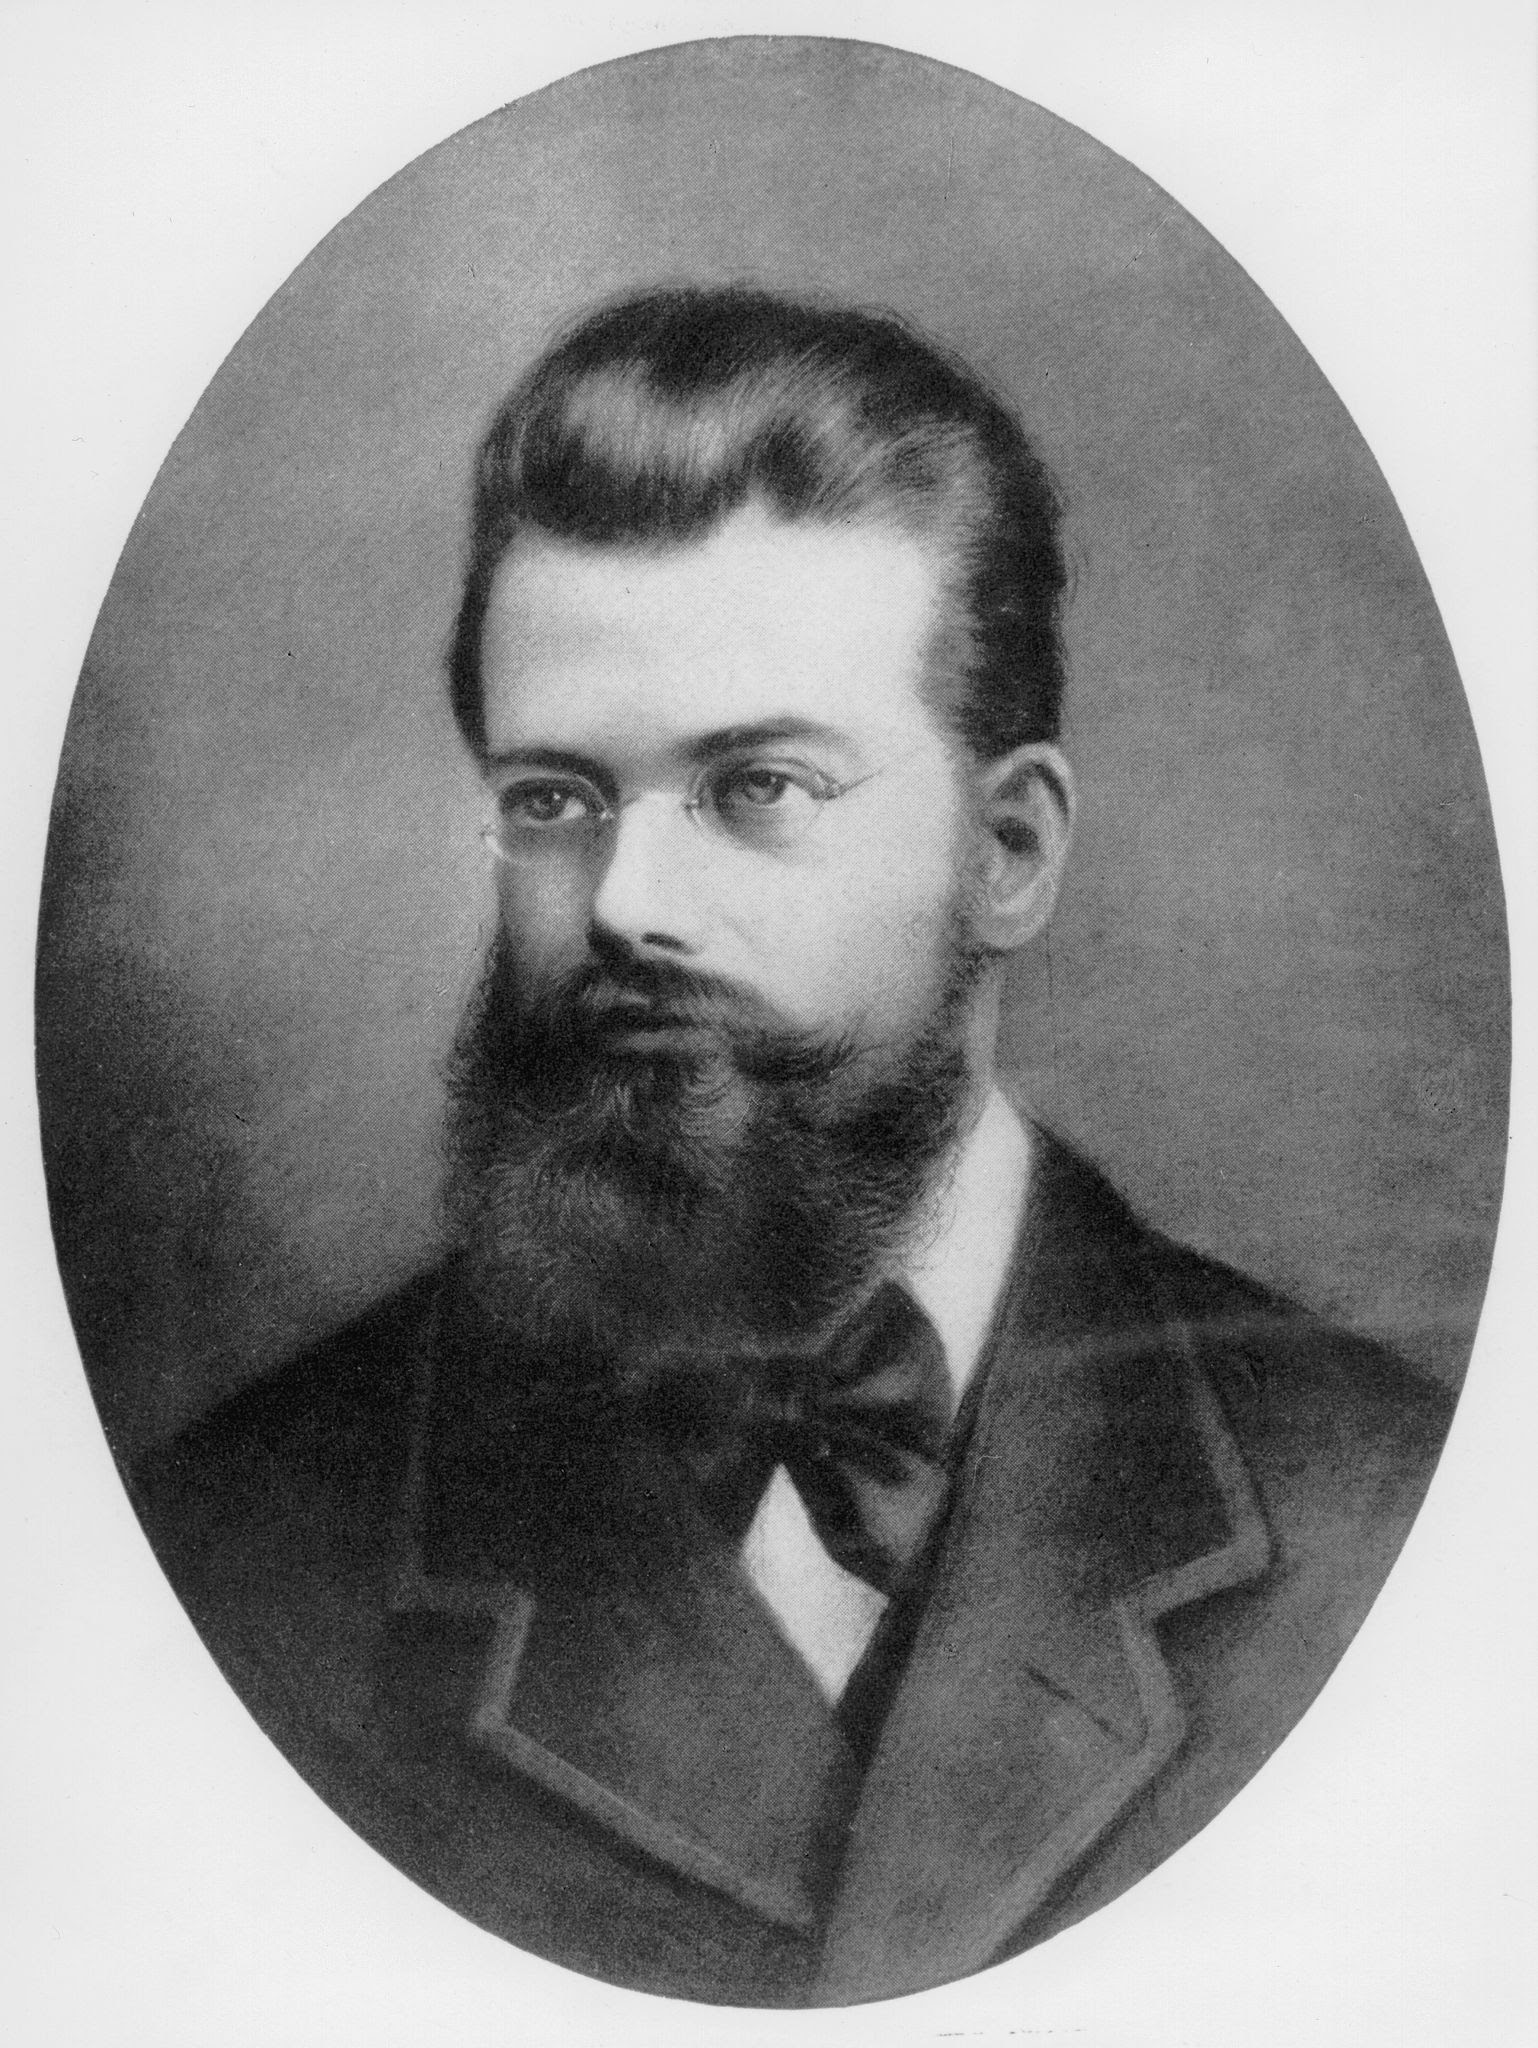
\includegraphics[scale=0.1]{Figures/boltzmann.jpeg}
  \end{center}
  \caption{picture of the magestic Boltzmann}
  \label{fig:boltzmann papa}
  \end{figure}
  

  \subsection{Boltzmann equation}%
    \label{sub:Boltzmann equation}
   
   The boltzmann equation reads, 

   \begin{align}
    \label{boltzmann equation}
    \frac{\partial f}{\partial t} &= - \frac{\textbf{p}}{m} \cdot \nabla_x
     f - m \textbf{a} \cdot \nabla_p f, 
   \end{align}
   Here we make the assumption that the system of interest is in the
   non-relativistic case and under the unperturbed FLRW metric. 

   And note that we can rewrite (\ref{Boltzmann equation}) in two cases, 
   \begin{align}
   \begin{cases} 
     \frac{\mathrm{d}f}{\mathrm{d}t} = \frac{\partial f}{\partial
     t} + x \cdot \nabla_x f = \textbf{p} \cdot \nabla_x f, &\textnormal{
     number conserved case} \\ 
     \frac{\mathrm{d}f}{\mathrm{d}t} =
     \underbrace{C[f]}_{\textrm{collision terms}} &\textnormal{number
     not conserved case}
   \end{cases}
    \end{align}

    For the 1st case, we shall get 
    \begin{align}
      \label{first case beyond}
      \frac{\mathrm{d}n_1}{\mathrm{d}t} + 3 H n_1 = 0 \implies n_1
      \propto a^{-3} 
    \end{align}
    and for the 2nd we get 
    \begin{align}
      \label{second case beyond}
      a^{-3} \frac{\mathrm{d}N_1}{\mathrm{d}t} = C_1 [ \{ n_j \} ].
    \end{align}
    For example, we can take the collision terms as 
    \begin{align}
      \label{collison term example}
       a^{-3} \frac{\mathrm{d}N_1}{\mathrm{d}t} = - \alpha
       n_1 n_2 + \beta  n_3 n_4
    \end{align}, where \( \alpha = \langle \sigma \nu \rangle,
    \hspace{0.1cm} \beta = \bigg( \frac{n_1 n_2}{n_3 n_4}
    \bigg)_{eq} \alpha     \).

    And now if we make a change of variable \( N_i \equiv
    \frac{m_i}{s} (s \propto a^{-3} ), \Gamma_{\gamma} \equiv m_2 \langle
    \sigma \nu  \rangle  = n_2 \alpha\), these are at the same time
    ansatz, 
we can express (\ref{collision term example}) as, 
\begin{align}
  \label{neater collision term}
  \frac{\mathrm{d} \mathrm{ln}(N_i)}{\mathrm{d}\mathrm{ln}(a)}  = \frac{- \Gamma_1}{H} \bigg[ 1 -
  \bigg(\frac{N_1 N_2}{N_3 N_4} \bigg)_{eq} \bigg( \frac{N_3 N_4}{N_1
  N_2} \bigg)  \bigg] 
\end{align}

And now notice in the limit \( H \ll \Gamma_{1} \), 
we have 
\begin{align}
   \label{H << gamma}
  \cancelto{0}{- \frac{H}{\Gamma_1}  \frac{\mathrm{d}
  \mathrm{ln}(N_i)}{\mathrm{d}\mathrm{ln}(a)}}  = \bigg[ 1 -
  \bigg(\frac{N_1 N_2}{N_3 N_4} \bigg)_{eq} \bigg( \frac{N_3 N_4}{N_1
  N_2} \bigg)  \bigg] 
\end{align}

and if in the limit \( \Gamma \ll H  \),
we have
\begin{align}
  \label{gamma << H}
  \frac{\mathrm{d}
  \mathrm{ln}(N_i)}{\mathrm{d}\mathrm{ln}(a)} = 0
\end{align}, this implies \( N_i \) a constant, i.e. freeze-out of species
\( N_i \).

\subsection{Dark matter}%
  \label{sub:Dark matter}
  Now we look into the behaviour of Boltzmann equation for dark matter
  (assuming WIMP-like particle), which the relevant interaction should
  take the form 
  \begin{align}
    \label{WIMP interaction}
    X + \bar{X} \to l + \bar{l}
  \end{align}
  and note that it should be much simpler as it we have the major
  assumptions (i) non-interacting; (ii) non-relativistic; (iii) these
  light particles (\( l, \bar{l} \)) are tightly coupled to the plasma of
  charged particles in the early Universe (which calls for
  \textit{tightly-coupled approximation}); (iv) these light particles
  are in equilibrium at later stage, \( n_l = n_{l}^{eq} \). We are also
  interested in predicting the relic-abundance for WIMP. 

  So using \( N_{X}^{eq} \equiv n_{X}^{eq}/s \), the Boltzmann equation
  becomes
  \begin{align}
    \label{WIMP Boltzmann}
    a^{-3} \frac{\mathrm{d}(n_x a^{-3} )}{\mathrm{d}t} &= - \langle
    \sigma \nu \rangle \bigg( n_{X}^{2} - (n_{X}^{(eq)})^2 \bigg) 
  \end{align}
  To make our lives simpler, turns out we need to make the change of
  variable \( Y \equiv n_X / T^3 \). And also with the assumption
  \( T \propto a^{-1}  \), then 
  \begin{align}
    \label{change to Y WIMP Boltzmann }
   \frac{\mathrm{d}Y}{\mathrm{d}t} &= - \langle \sigma \nu \rangle
    T^{3} \bigg( Y^2 - (Y_{X}^{(eq)})^2 \bigg)  
  \end{align}
  And again make a change of variable \( x \equiv M_x /T \) to get 
  \begin{align}
    \label{change to x}
    \frac{\mathrm{d}x}{\mathrm{d}t} &=
    \frac{\mathrm{d}}{\mathrm{d}t} \bigg( \frac{M_x}{T} \bigg) =
    \frac{-1}{T} \frac{\mathrm{d}T}{\mathrm{d}t}x
  \end{align}, and remembering \( T \propto a^{-1}  \), we conclude
  with 
  \begin{align}
    \label{ooof}
    \frac{\mathrm{d}x}{\mathrm{d}t} \approx H x
  \end{align}
\hl{The above equation is useful to remember.}  
Now we plug all these in to the Boltzmann equation, it will reduce to
the Riccati equation: 
\begin{align}
  \label{Riccati equation}
  \frac{\mathrm{d}Y}{\mathrm{d}x} &=  - \frac{\lambda}{x^2} \bigg( Y^2
  - (Y^{(eq)})^2\bigg)  
\end{align}, where 
\begin{align}
  \label{lambdaaaa}
  \lambda \equiv \frac{M_{X}^{3} \langle \sigma \nu \rangle  }{H(M_X)}
\end{align}

To obtain a solution, we assume (otherwise numerical) the freeze-out occurs
at some time \(  x = x_f \). and the integration becomes 
\begin{align}
  \label{integration of Riccati equation}
  \int_{Y^f}^{Y^{\infty}} \frac{\dd[]{Y}}{Y^2} &=  -
  \int_{x_f}^{\infty} \dd[]{}x \frac{\lambda}{x^2} \\ 
  \frac{1}{Y^{\infty}} - \frac{1}{Y^f} &= \frac{\lambda}{x_f}. 
\end{align}
And assuming \( Y^f \gg Y^{\infty} \), 
we arrive at 
\begin{align}
  \label{solution to Riccati equation}
  Y^{\infty} \approx \frac{x_f}{\lambda}. 
\end{align}. \hl{The typical } \( x_f \sim 10 \)   

\section{Hydrogen recombination}%
  \label{sub:Hydrogen recombination}

After BBN (and photon epoch), we get the recombination period, which
happens around  \hl{$ T > 1 \mathrm{eV}$ }. And the relevant processes
are 
\begin{align}
  \label{hyrogen recombination processes}
  e^- + p^+ &\leftrightarrow H + \gamma \\ 
  \label{photon scattering}
  e^- + \gamma &\leftrightarrow e^- + \gamma 
\end{align}
  
And when electrons and protons combine to form neutral atoms, now the density
of free electrons significantly drops, and the photons can now travel
through freely without scattering via process (\ref{photon scattering}).
This is also where CMB photons are "generated". 

\textbf{Remarks: } The term "recombination" is a bit of misnomer as this is
the first time that electrons and protons combine into neutral hydrogen.

\subsection{free electron fraction}%
  \label{sub:free electron fraction}
  The main  goal here is to predict the free electron fraction, \( X_e
  \equiv n_e / n_b \), where \( n_b \) denotes the density of baryons.
  Here we are also assuming (i) non-relativistic limit, which implies 
  \begin{align}
    \label{equilibrium abundancces of species in hydrogen
    recombination}
    n_{i}^{eq} &= g_i \bigg(\frac{m_i T}{2 \pi} \bigg)^{3/2} \mathrm{exp}
    \hspace{0.1cm} \bigg( \frac{\mu_i - m_i}{T} \bigg); 
  \end{align}
(ii) the relevant species are \( i = \{ e, p, H \} \)

  And note that the chemical potentials of the three species is \( \mu_p +
  \mu_e = \mu_H \)

With these, we can get the ratio as, 
\begin{align}
  \label{ratio hydrogen over electrons and protons}
  \frac{n_{H}^{eq}}{n_{e}^{eq} n_{p}^{eq}} &= \frac{g_H}{g_e g_p} \bigg(
  \frac{m_H}{m_e m_p} \frac{2\pi}{T} \bigg)^{3/2} \mathrm{exp}
  \hspace{0.1cm} \bigg( \frac{m_p + m_e - m_H}{T} \bigg) 
\end{align}, we can also further make assumptions 
\begin{enumerate}
  \item[\circ] \( m_H \approx m_p \), but for only the prefactor, 
  \item[\circ]  no net charge, \( n_e = n_p \)
  \item[\circ] the binding energy of hydrogen is \( B_H = m_p + m_e - m_H
  = 13.6 eV\)
  \item[\circ] number of dof: \( g_p = g_e = 2, g_H = 4 \)
\end{enumerate}

Then everything will be simplified as 
\begin{align}
  \label{simplified ratio}
  \bigg(\frac{n_H}{n_{e}^{2}} \bigg)_{eq}  &=
  \bigg(\frac{2\pi}{m_e T} \bigg)^{3/2} e^{B_H/T}  
\end{align}
We can now use this equation to keep track of the free electron fraction. To
do so, we first write the number density of baryon as: 
\begin{align}
  \label{number density of baryon }
  n_b = \eta n_{\gamma} = \eta \frac{2 \zeta(3)}{\pi^2} T^{3} 
\end{align}, where \( \eta \) is the baryon-to-photon ratio that is
determined observationally.

and the with the following assumption 
\begin{align}
  \label{assumption on number density of baryons}
  n_b \approx n_p + n_H = n_e + n_H 
\end{align}
Putting the (\ref{assumption on number density of baryons}) and (\ref{number
density of baryon }) together, we get 
\begin{align}
  \label{mix of densities}
  \bigg( \frac{1-X_e}{X_{e}^{2}} \bigg)_{eq} &=
  \frac{n_H}{n_{e}^{2}} n_b
\end{align}
and finally plug (\ref{mix of densities}) to (\ref{simplified ratio}), we
obtain the \textit{Saha equation}, 
\begin{align}
  \label{Saha equation}
  \bigg(\frac{1-X_e}{X_{e}^{2}} \bigg)_{eq} &= \eta \frac{2
  \zeta(3)}{\pi^2} \bigg(\frac{2\pi T}{m_e} \bigg)^{3/2} e^{B_H/T} 
\end{align}



\begin{figure}[h!]
\begin{center}
  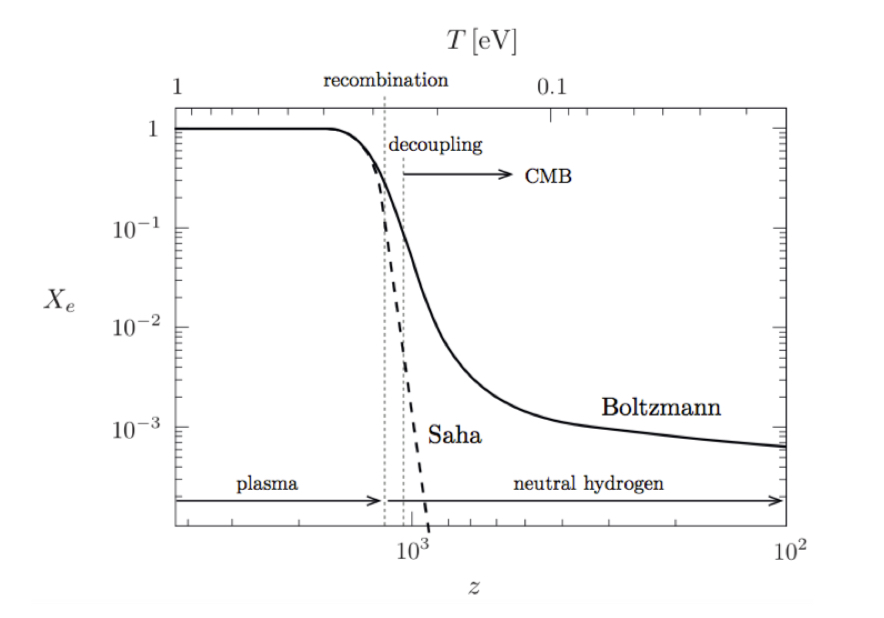
\includegraphics[scale=0.3]{Figures/Saha.jpeg}
\end{center}
\caption{The electron abundance as a function of redshift in the early
  Universe. The Saha equation under predicts the abundance left after
  recombination and decoupling. To get the right abundance, one must solve
  the Boltzmann equation numerically.}
\label{fig:Saha}
\end{figure}



\subsubsection{Quick redshift estimation}%
  \label{sub:Quick redshift estimation}
  For early universe era (up to recombination), we can abuse the
  relation \( T \propto a^{-1}  \), and say if we were to predict redshift
  of recombination, then we do 
  \begin{align}
    \label{redshift of recombination}
    T_{rec}  = T_0 ( 1 + z_{rec} )
  \end{align}, and note that \( T_0 \) is the temperature of CMB (2.71K).
  To further obtain the age, then we do \( a = (t/t_0)^{2/3} \), with t_0
  as age of the universe.
 
 \subsection{Photon decoupling}%
  \label{sub:Photon decoupling}
  To obtain the time for photon decoupling, which happens right after
  recombination, exactly when 
  \begin{align}
    \label{photon decoupling}
    \Gamma_{\gamma}(T_{rec}) \approx H(T_{dec})
  \end{align}, and that the we know the cross-section for Thomson scattering
  to be \( \sigma_T \approx 2 \times 10^{-3} \mathrm{MeV}^{-2}  \). Thus
  we can estimate with
  \begin{align}
    \label{estimating photon decoupling}
    \Gamma_{\gamma} \approx n_e \sigma_T \approx H(T_{dec})
  \end{align}, which yields a temperature of \( T_{dec} \approx 0.27 eV\)

  \section{Jesus christ is BBN (Not Julio)}%
    \label{sec:Jesus christ is BBN (Not Julio)}
   
   Let us now go back in time (bruh moment), at BBN period \( T_{BBN}
   \approx 1 \mathrm{MeV} \), and here we will focus on how helium is
   synthesised. 

   \subsection{Neutron abundance in equlibrium}%
    \label{sub:Neutron abundance in equlibrium}
  
    The relevant process here is the weak interaction
    \begin{align}
      \label{neutron abundance}
      p^+ + e^- \leftrightarrow n + \nu_e
    \end{align}, you may ask why this is important. And the answer
    is because Helium requires neutron to form simply. 
   
    The ratio of proton over neutron in equilibrium is thus 
    \begin{align}
      \label{ratio in neutron abundance}
      \frac{n_{p}^{eq}}{n_{n}^{eq}} \approx \bigg(\frac{m_n}{m_p}
      \bigg)^{3/2} e^{(m_n-m_p)/T} 
    \end{align}, the assumption we made for the approximation here is that the
neutrinos have zero chemical potential, and of course the non-relativistic
limit setting to get to (\ref{ratio in neutron abundance}), we can do the
same approximation we did for the prefactor on the \textnormal{R.H.S.},
setting \( m_n = m_p \) and further reducing it to the value such that we can
compute, the ratio readily. Though if we consider the limits for \( T \), we
will begin to notice that around \( T < T_{BBN} \approx 1 \mathrm{MeV}
\), the neutrons starts to be scarce, i.e. the ration becomes away (much
larger) than 1. Thus this calls for a look into different processes
that crossing our fingers it will produce more neutrons. 

\subsection{The deuterium bottleneck}%
  \label{sub:The deuterium bottleneck}
  The relevant process here is 
  \begin{align}
    \label{deuterium process}
    n + p^+ \leftrightarrow D + \gamma
  \end{align}, 
  And with Deuterium, we can further produce Helium via the following
  two processes, 
  \begin{align}
    \label{helium processes 1}
    D + p^+ &\leftrightarrow^3 \mathrm{He} + \gamma \\ 
    \label{helium processes 2}D + ^3\mathrm{He} &\leftrightarrow^4 \mathrm{He} + p^+
  \end{align}

  So the corresponding process, under the assumptions on the chemical
  potential \( \mu_{\gamma} = 0 \implies \mu_{n} + \mu_{p} = \mu_{D}
  \), we obtain 
  \begin{align}
    \label{deuterium ratio}
   \frac{n_{D}^{eq}}{n_{n}^{eq} n_{p}^{eq}} &= \frac{g_D}{g_n g_p} \bigg(
  \frac{m_D}{m_e m_p} \frac{2\pi}{T} \bigg)^{3/2} \mathrm{exp}
  \hspace{0.1cm} \bigg( \frac{m_n + m_p - m_D}{T} \bigg) 
  \end{align}, the dof in this expression are naturally \( g_D = 3, \) and
  \( g_n = g_p = 2 \), and the mass assumptions are \( m_D \approx
  2m_n \approx 2 m_p \).
  Then we can reduce (\ref{}) to 
  \begin{align}
    \label{simplified deuterium ratio}
   \frac{n_{D}^{eq}}{n_{p}^{eq}} &= \frac{3}{4} n_{n}^{eq}
    \bigg(\frac{4\pi}{m_p T} \bigg)^{3/2} \mathrm{exp} \hspace{0.1cm}
    \bigg( \frac{B_D}{T} \bigg)   
  \end{align}
  
  Again, we can pack the previous equation (\ref{simplified deuterium
  ratio}) to a nicer compact form by first introucing, 
  \begin{align}
    \label{neutron number density in terms of gamma again}
    n_n \approx n_b = \eta n_{\gamma} = \eta \frac{2
    \zeta(3)}{\pi^2}T^3, 
  \end{align} and shove this to (\ref{simplified deuterium ratio})
  and obtain 
  \begin{align}
    \label{Deuterium Saha equation}
    \frac{n_{D}^{eq}}{n_{p}^{eq}} \approx \eta \bigg(\frac{T}{m_p}
    \bigg)^{3/2} \mathrm{exp} \hspace{0.1cm} \bigg( \frac{B_D}{T} \bigg) 
  \end{align}
  
  Ideally we want the ratio to be large, which is in the limit \( T \ll B_D
  \), thus it has to wait for the Universe to cool down
  sufficiently, and thus called the "deuterium bottleneck", as this
  heavily decides the rate of formation of helium.
  \subsubsection{Neutrons out of equilibrium}%
    \label{sub:Neutrons out of equilibrium}
    To obtain the neutron fraction, we define 
    \begin{align}
      \label{neutron fraction}
      X_{n} \equiv \frac{n_{n}}{n_{n} n_{p}}, 
    \end{align} and then we can use the previous (\ref{ratio in neutron
    abundance}) to obtain (some steps omitted, primarily dividing both
    terms by \( n_{p}^{eq} \)), 
    \begin{align}
      \label{final form for neutorn fraction}
      X_{n}^{eq}(T) &= \frac{e^{-(m_n - m_p)/T} }{1 + e^{-(m_n - m_p)/T} } 
    \end{align}, we can take \( T = T_{rec} \approx 0.8
    \mathrm{MeV} \) to obtain \( X_{n}^{eq}(T_{dec}) = 0.17 \)
    
    \subsubsection{Neutron decay}%
      \label{sub:Neutron decay}
      After the freeze-out of neutron, neutron start to decay via weak
      interactions, 
      \begin{align}
        \label{neutron decay}
        n \rightarrow p^+ + e^- + \bar{\nu}_{e}
      \end{align}
      And the decay goes exponentially as 
      \begin{align}
        \label{exponential decay of neutron}
        X_{n}(t) &=  0.17 e^{-t/\tau_n},
      \end{align} with \( \tau_{n} = 889.7 \hspace{0.1cm} \mathrm{s}
      \).


    \subsection{Helium fusion}%
      \label{sub:Helium fusion}

      Now we are in the position to tackle the production of helium
      in the early Universe, and note that the reaction paths we have
      gone through are the dominant processes that produces helium
      efficiently, for they are two-body interactions. So at \( T_{nuc}
      \approx 0.06 \mathrm{MeV}\), we get what we wish for - Helium
      production!

      And note that to obtain the time estimate, we can make use of
      scaling of temperature of the Universe with time as \( T
      \propto t^{-1/2}  \), and get 

      \begin{align}
        \label{time T relation on helium production}
        \frac{T}{1 \hspace{0.1cm} \mathrm{MeV}} \approx 1.5
        g_{\star}^{-1/4} \bigg(\frac{1
        \hspace{0.1cm}\mathrm{s}}{t} \bigg)^{1/2}  
      \end{align}

    From (\ref{time T relation on helium production}), if we plug in what
    we have found earlier that \( T_{nuc} \approx 0.06 \hspace{0.1cm}
    \mathrm{MeV} \), and we should get \( t_{nuc} \approx 330
    \hspace{0.1cm}\mathrm{s} \). And if we were to use
    (\ref{exponential decay of neutron}) with this time. We will get 
    \begin{align}
      \label{estimated abundance of neutron}
      X_{n}(t_{nuc}) &= 0.17 e^{-t_{nuc}/\tau_{n}} \approx
      \frac{1}{8}  
    \end{align}
    And now notice the following three items 
    \begin{enumerate}
      \item[\it 1.] \( n_{\mathrm{He}} = \frac{1}{2}
      n_{n}(t_{nuc}) \), that each helium requires 2 neutron to form. 
      \item[\it 2.] \( n_{H} = n_{p} \), the abundance of hydrogen
      is just abundance of proton (indirect assumption of no net charge
      and number conservation). 
    \end{enumerate}
    So finally we get from
    \begin{align}
      \label{abundance ratio}
      \frac{n_{\mathrm{He}}}{n_{\mathrm{H}}} &=
      \frac{n_{\mathrm{He}}}{n_{\mathrm{p}}} \approx
      \frac{\frac{1}{2} X_{n}(t_{nuc})}{1 - X_{n}(t_{nuc})}
      \approx \frac{1}{2} X_{n}(t_{nuc}) \sim \frac{1}{16}
    \end{align}
    and abundance by mass is 
    \begin{align}
      \label{abundance of helium by mass}
      \frac{4 m_{\mathrm{He}}}{m_{\mathrm{H}}} &=  \frac{1}{4} 
    \end{align}

    \begin{figure}[h!]
    \begin{center}
      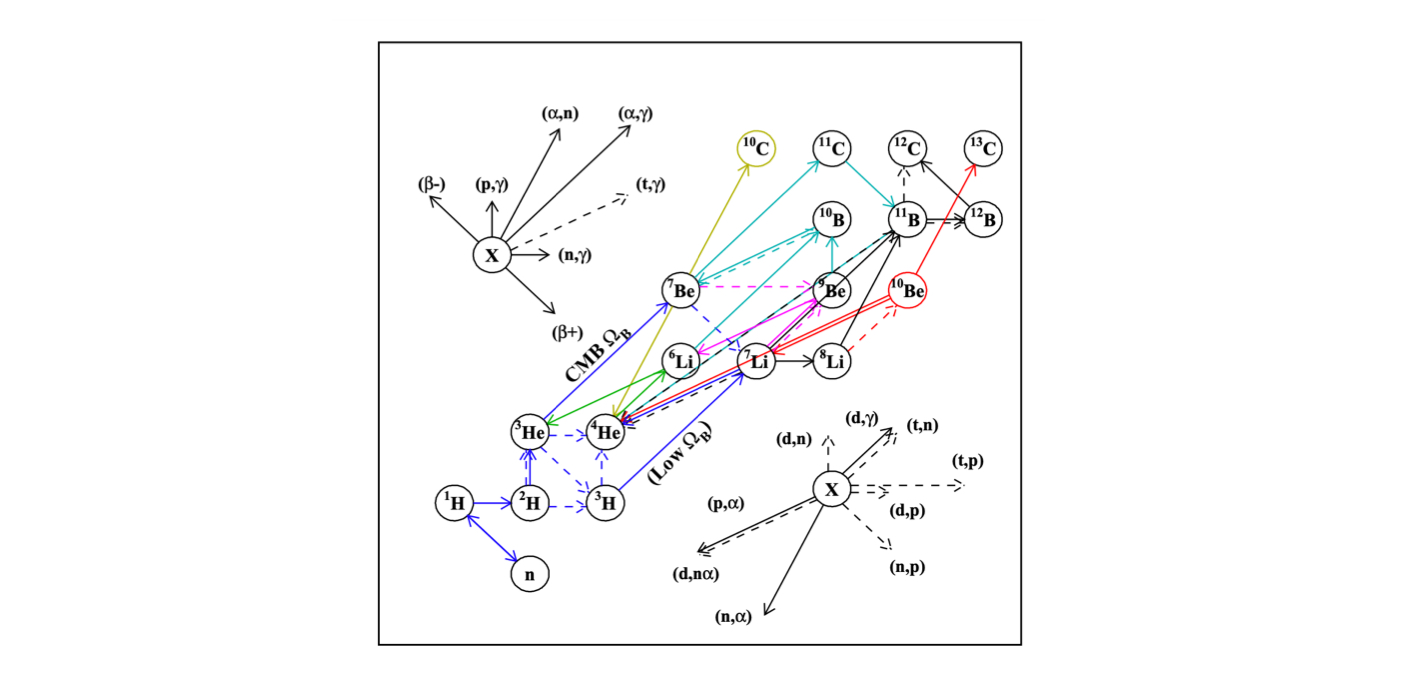
\includegraphics[scale=0.3]{Figures/cursedchain.jpeg}
    \end{center}
    \caption{Chain of the \textit{cursed} BBN reactions.}
    \label{fig:cursedchain}
    \end{figure}
    
    \begin{figure}[h!]
    \begin{center}
      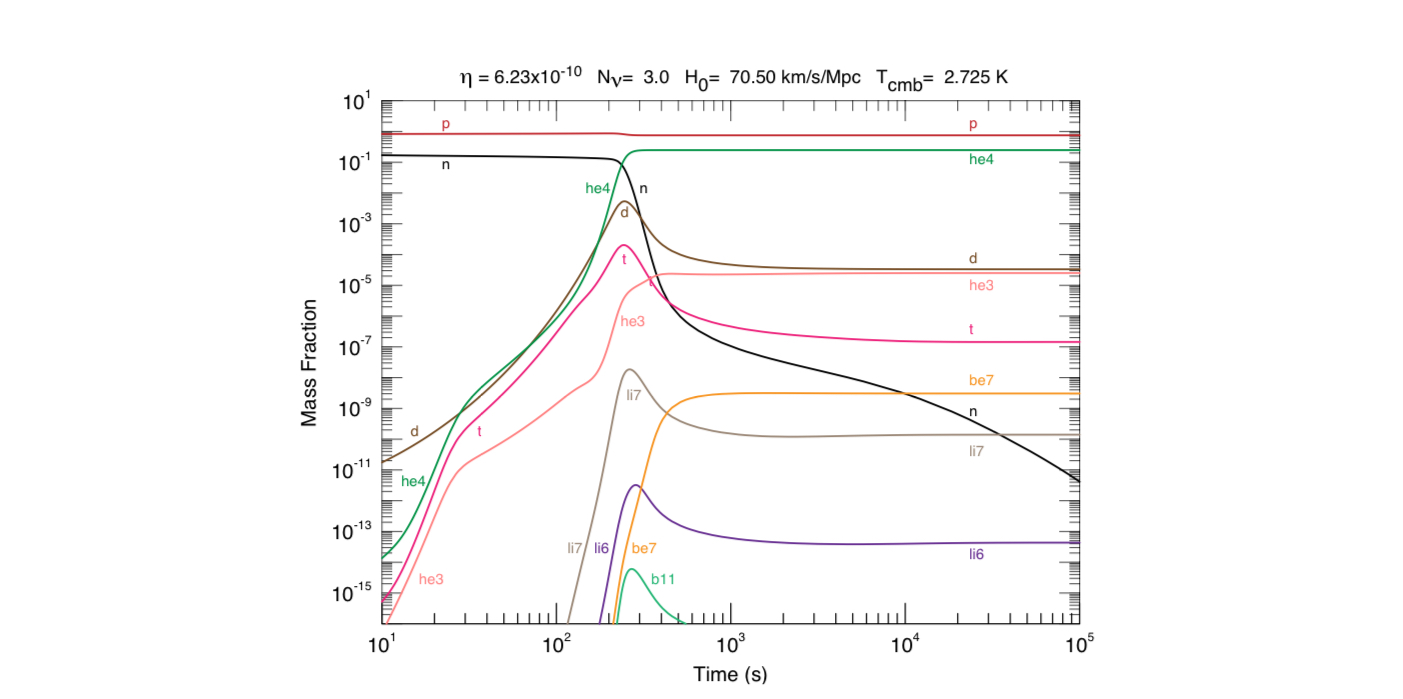
\includegraphics[scale=0.3]{Figures/abundance.jpeg}
    \end{center}
    \caption{Predicted mass fraction by element from Big Bang
      nucleosynthesis chain of interactions.}
    \label{fig:abundance.jpeg}
    \end{figure}
    



  \subsection{Big review of Beyond Equilibrium in general}%
    \label{sub:Big review of Beyond Equilibrium in general}
    Note that for a given reaction, and if assumed non-relativistic
    limit. 
    \begin{align}
      \label{processeca}
      A + B \leftrightarrow C + D
    \end{align}
    We can immediately obtain the equation below, 
    \begin{align}
      \label{processeca ABCD}
   \frac{n_{C}^{eq}}{n_{A}^{eq} n_{B}^{eq}} &= \frac{g_C}{g_A g_B} \bigg(
  \frac{m_C}{m_e m_p} \frac{2\pi}{T} \bigg)^{3/2} \mathrm{exp}
  \hspace{0.1cm} \bigg( \frac{m_A + m_B - m_C}{T} \bigg) 
    \end{align}, with the assumption that D is just photon, and next we
    compute for the dof and prefactor masses with given assumptions
    for the corresponding species. 
   
\section{The Boltzmann equation}%
  \label{sec:The Boltzmann equation}
  
In this section, we aim to recover the tiny
\textbf{inhomogeneities} of the CMB at the scales of \( \mu \mathrm{K}
\), which originates from the quantum fluctuations of the inflationary
potential.
\subsection{Boltzmann equation for perturbations}%
  \label{sub:Boltzmann equation for perturbations}
  
  

  At decoupling \( z \sim 1100 \), we have the particles soup 
  \begin{align}
    \label{z 1100 particle soup}
    \rho, e^- \nu, \gamma, \mathrm{DM}
  \end{align}
The big picture of the system of (Boltzmann) equations we are solving is
  as follows, 
  \begin{figure}[h!]
  \begin{center}
    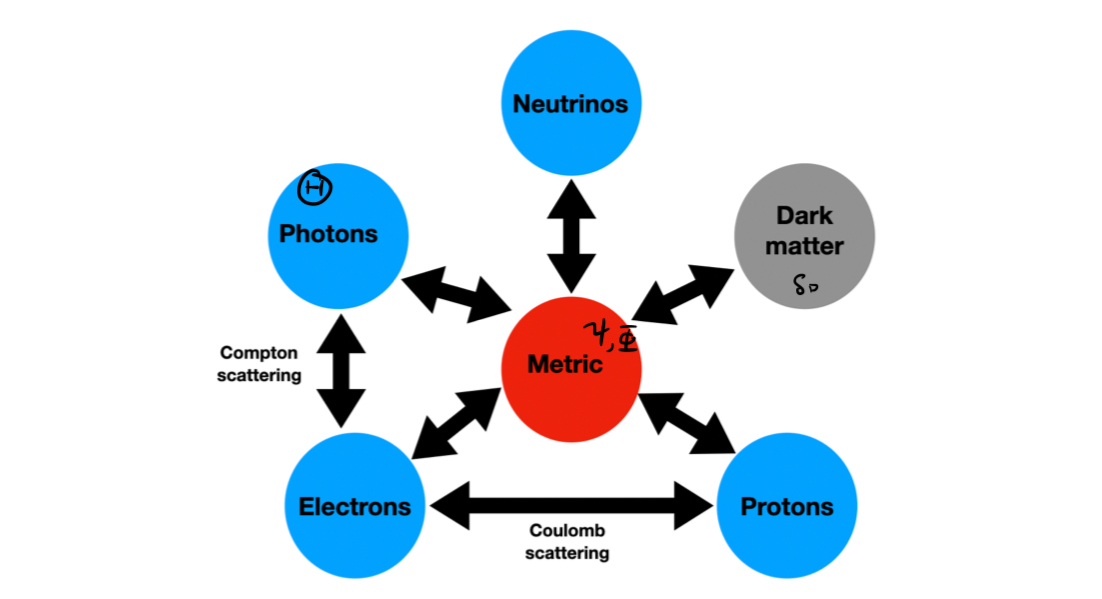
\includegraphics[scale=0.3]{Figures/boltzmannspread.jpeg}
  \end{center}
  \caption{Species present in the Universe at the time of
    recombination and their interactions.}
  \label{fig:}
  \end{figure}

  and we introduce the metric perturbations 
  \begin{align}
    \label{metric perturbations}
    g_{00} = -1 - 2 \Psi(\textbf{x}, t), \hspace{0.5cm} g_{0i} = 0,
    \hspace{0.5cm}g_{ij} = a^{2} \delta_{ij}^{} ( 1 + 2
    \Phi(\textbf{x, t}) )  
  \end{align}. 

  It is also necessary to introduce the geodesic deviation to the system of
  equations we are trying to solve, as we have to solve for \( f_i \) in
  \( g_{\mu \nu} \): \( \frac{\mathrm{d}f_i}{\mathrm{d}t} = C[f_i,
  f_j]. 
  \) It is now instructive to gain more intuition about the
  aforementioned Boltzmann equation. 

  \subsection{Intuition on Boltzmann equation through SHO}%
    \label{sub:Intuition on Boltzmann equation through SHO}
  We can quickly gain some intuition on Boltzmann equation through
  SHO system, with the energy defined as the usual 
  \begin{align}
    \label{SHO energy}
    E &= \frac{p^2}{2m} + \frac{1}{2} k x^{2}   
  \end{align}
  and note that 
  \begin{align}
    \label{SHO equations}
    \frac{\mathrm{d}x}{\mathrm{d}t} = \frac{\rho}{m}, \hspace{0.5cm}
    \frac{\mathrm{d}p}{\mathrm{d}t} = -kx
  \end{align}
  Given there is no collision term, we can then write the Boltzmann
  equation as, 
  \begin{align}
    \label{SHO boltzmann}
    \frac{\mathrm{d}f}{\mathrm{d}t} &= \frac{\partial f}{\partial t} +
    \frac{\partial f}{\partial x} \frac{\mathrm{d}x}{\mathrm{d}t}
    + \frac{\partial f}{\partial p}
    \frac{\mathrm{d}p}{\mathrm{d}t} = 0 \\ 
    \implies \frac{\mathrm{d}f}{\mathrm{d}t} &=  \frac{\partial
    f}{\partial t} + \frac{p}{m} \frac{\partial f}{\partial x}  - k
    x \frac{\partial f}{\partial p} = 0 
  \end{align}, where we have simply used (\ref{SHO equations}) to obtain
  the final expression for (\ref{SHO boltzmann}).
  
  In order to further obtain more results, we need initial condition
  of the particle, which we now impose they are at equilibrium. 

  \textbf{Equilibrium: } Now we suppose the system is in
  equilibrium, then we have \( \partial_{}^{} f / \partial_{}^{}t = 0
  \). Then we will get 
  \begin{align}
    \label{SHO equlibrium distribution}
    f(x, p) &= f_{eq}(E[p, x]) 
  \end{align}, this means the system only depends on the function of
  the energy of the particle, then we can replace the total derivative
  w.r.t E instead of t. The new expression becomes 
  \begin{align}
    \label{new expression for SHO}
    \frac{p}{m}\frac{\partial f}{\partial x}  - k x \frac{\partial
    f}{\partial p} &= \frac{\mathrm{d}f}{\mathrm{d}E} \bigg[
    \frac{p}{m} \frac{\partial E}{\partial x} - k x \frac{\partial
    E}{\partial p}  \bigg]   = 0 
  \end{align}
  
  \subsection{Photons, electrons, and metrics relations}%
    \label{sub:Photons, electrons, and metrics relations}
    In this section, we will probe the influence in interactions between
    electrons, photons and metrics to the Boltzmann equation. Note that
    the interaction goes as \( \mathrm{electrons} \leftrightarrow
    \mathrm{photons} \leftrightarrow \mathrm{the metric}\). Now the
    relevant interaction of photon and electrons are via Compton
    scattering. 
    \begin{align}
      \label{Compton scattering}
      e^- + \gamma \leftrightarrow e^- + \gamma
    \end{align}, whereby a photon encounters an electron and they
    exchange energy momentum. 
    
    Since we are trying to get something similar to that of (\ref{new
    expression for SHO}), we need to find the momentum of the photon
    first, which can be done by 
    \begin{align}
      \label{momentum with affine parameter}
      P^{\mu} \equiv \frac{\mathrm{d}x^{\mu} }{\mathrm{d}\lambda}  
    \end{align}
    and we have the usual normalisation on the momentum in GR as 
    \begin{align}
      \label{momentum constraint}
      P^2 \equiv g_{\mu \nu} P^{\mu} P^{\nu} = - (1 +
      2\Psi)(P^{0} )^2 + p^2 = 0.
    \end{align}
    So in the end we have the spatial and temporal part of the momentum
    separated, with 
    \begin{align}
      \label{spatial momentum}
      p^2 = g_{ij} P^{i} P^{j}, \hspace{0.5cm} p^{i} &= p
      \hat{p}^{i}, \hspace{0.5cm} \delta_{ij}^{}
      \hat{p}^{i} \hat{p}^{j} = 1   
    \end{align} 
   After some equation merging and approximation, we will arrive at 
   \begin{align}
    \label{affine momentum}
     P^{i} &= p \hat{p}^{i} \frac{(1 - \Phi)}{a}   
   \end{align}
   Packing everything into the Boltzmann equation 
   \begin{align}
    \label{metric to Boltzmann equation}
     \frac{\mathrm{d}f}{\mathrm{d}t} = \frac{\partial f}{\partial
     t} + \frac{\partial f}{\partial x^{i} }
     \frac{\mathrm{d}x^{i} }{\mathrm{d}t} + \frac{\partial f}{\partial
     p} \frac{\mathrm{d}p}{\mathrm{d}t} +
     \underbrace{\frac{\partial f}{\partial \hat{p}^{i} }
     \frac{\mathrm{d} \hat{p}^{i} }{\mathrm{d}t}
     }_{\textrm{2nd order}} = C[f] 
   \end{align}, where we can drop the 2nd order as we wish.

   With this, we have obtained 
   \begin{align}
    \label{v in t}
     \frac{\mathrm{d}x^{i} }{\mathrm{d}t} =
     \frac{\mathrm{d}x^{i}
     }{\mathrm{d}\lambda}\frac{1}{\mathrm{d}t /
     \mathrm{d}\lambda} = \frac{P^{i} }{P^{0} } \approx
     \frac{\hat{p}^{i} }{a} ( 1 + \Phi - \Psi ) <
     \frac{\hat{p}^{i} }{a},
   \end{align} note that with this expression, it means the photon
   climbs out of an over-dense region, and when \( \Psi < 0,  \) and \(
   \Phi > 0 \), it slows down
   And the Boltzmann equation now reads 
   \begin{align}
    \label{Boltzmann equation after metric and photon}
     \frac{\mathrm{d}f}{\mathrm{d}t} = \frac{\partial f}{\partial
     t} + \frac{\partial f}{\partial x^{i} } \cdot \frac{\hat{p}^{i} }{a} +
     \frac{\partial f}{\partial p} \frac{\mathrm{d}p}{\mathrm{d}t}
   \end{align}

  \subsection{Implementing geodesic equation}%
    \label{sub:Implementing geodesic equation}
    
    After going through the calculations on previous sections, we are in
    the position to calculate the 3rd term of (\ref{Boltzmann equation
    after metric and photon}). 
    We can begin with the time component of the geodesic equation, 
    \begin{align}
      \label{time component of geodesic equation}
      \frac{\mathrm{d} P^{0} }{\mathrm{d}\lambda} &= -
      \Gamma_{\alpha \beta}^{0} P^{\alpha} P^{\beta},   
    \end{align} 

      And we can plug (\ref{affine momentum}) to (\ref{time component of
      geodesic equation}) and expand the total derivative of \( \Psi \)
      w.r.t time and obtain 
      \begin{align}
        \label{dp/dt in phi}
        \frac{\mathrm{d} p}{\mathrm{d}t} &= p \bigg\{ \frac{\partial
        \Psi}{\partial t}  + \frac{\hat{p}^{i} }{a} \frac{\partial
        \Psi}{\partial x^{i} }   \bigg\}  -
        \Gamma_{\alpha\beta}^{0} \frac{P^{\alpha} P^{\beta}  }{p}
        (1 + 2\Psi).
      \end{align}

      Further manipulation should get us 
      \begin{align}
        \label{final boltzmann for metric photon}
        \frac{\mathrm{d}f}{\mathrm{d}t}  = \frac{\partial f}{\partial
        t} + \frac{\partial f}{\partial x^{i} } \cdot
        \frac{\hat{p}^{i} }{a} - p \frac{\partial f}{\partial p}
        \bigg[ H + \frac{\partial \Phi}{\partial t}  +
        \frac{\hat{p}^{i} }{a}\cdot \frac{\partial \Psi}{\partial
        x^{i} }  \bigg]  
      \end{align}

      \subsection{Photon perturbation}%
        \label{sub:Photon perturbation}
        Next, we shall focus on \( \mathrm{d}f/\mathrm{d}t \), to do
        so, we assume the distribution function is to 0th-order a BE
        equilibrium function with \( \mu = 0 \).



        Next, We define the photon temperature perturbation as 
        \begin{align}
          \label{photon perturbation}
          \Theta(\textbf{x}, \hat{p}, t) &= \frac{\delta
          T}{T}(\textbf{x}, \hat{p}, t)  
        \end{align}

        The distribution \( f(\textbf{x}, p, \hat{p}, t) \) now reads 
        \begin{align}
          \label{BE equilibrium distribution function}
          f(\textbf{x}, p, \hat{p}, t) = \bigg[\mathrm{exp}
          \hspace{0.1cm} \bigg\{ \frac{p}{T(t)[1 +
          \Theta(\textbf{x}, \hat{p}, t)]} \bigg\} - 1 \bigg]^{-1}
        \end{align}

        We then do 1st order expansion on this and get, 
        \begin{align}
          \label{1st order on f dist}
          f(\textbf{x}, p, \hat{p}, t) \approx f^{(0)} - p
          \frac{\partial f^{(0)} }{\partial p} \Theta.
        \end{align}

        At this point forward, we have to solve the Boltzmann
        equation \hl{order by order}.    

        \subsubsection{0th order}%
          \label{sub:0th order}
          At 0th order, there are no collisions, and the equation
          reads 
          \begin{align}
            \label{0th order of boltzmann}
            \frac{\mathrm{d}f^{(0)} }{\mathrm{d}t} = 0 \implies
            \frac{\mathrm{d}T}{T} = - \frac{\mathrm{d}a}{a}
          \end{align}, so we get \( T \propto a^{-1}  \). 

          \subsubsection{1st order}%
            \label{sub:1st order}
            At 1st order, we will get collision terms and the
            expression goes 
            \begin{align}
              \label{1st order of boltzmann}
              \frac{\mathrm{d}f^{(1)} }{\mathrm{d}t} = - p
              \frac{\partial f^{(0)} }{\partial p} \bigg[
              \frac{\partial \Theta}{\partial t} +
              \frac{\hat{p}^{i} }{a} \cdot \frac{\partial
              \Theta}{\partial x^{i} } + \frac{\partial
              \Phi}{\partial t} + \frac{\hat{p}^{i} }{a}\cdot
              \frac{\partial \Psi}{\partial x^{i} }  \bigg] =
              C[f(p)],
            \end{align} where the collision term here is the
            Compton scattering, which goes like 
            \begin{align}
              \label{compton scattering} 
              C[f(p)] = - p \frac{\partial f^{(0)} }{\partial p}
              n_{e} \sigma_{T}[\Theta_{0} - \Theta(\hat{p}) +
              \hat{p}\cdot \textbf{v}_{b}],
            \end{align} where 
            \begin{align}
              \label{theta0}
              \Theta_{0}(\textbf{x},t) \equiv \frac{1}{4 \pi}
              \int \dd[]{\Omega^{\prime} } \Theta (
              \hat{p}^{\prime}, \textbf{x},t).
            \end{align}
        Next we perform a change of variable \( a \mathrm{d} \eta
        = \mathrm{d}t\), i.e. the conformal time, to get 
        \begin{align}
          \label{change of var on 1st order of boltzmann}
          \Theta^{\prime} + \hat{p} \cdot \frac{\partial
          \Theta}{\partial x^{i} } + \Phi^{\prime} + \hat{p}^{i}
          \cdot \frac{\partial \Psi}{\partial x^{i} } = n_{e}
          \sigma_{T} a [\Theta_{0} - \Theta + \hat{p} \cdot
          \textbf{v}_{b}], 
        \end{align} where \( \Theta^{\prime} \) denotes
        derivative with respect to conformal time. 

        Next we perform \textit{Fourier transform}, via 
        \begin{align}
          \label{fourier transform on Theta}
          \Theta(\textbf{x}) &= \int \frac{\mathrm{d}^{3} k}{(2
          \pi)^{3}} e^{i \textbf{k} \cdot \textbf{x}}
          \tilde{\Theta}(\textbf{k}), 
        \end{align} which ultimately leads us to 

        \begin{align}
          \label{fourier boltzmann metric photon electron}
          \tilde{\Theta}^{\prime} + i k \mu \tilde{\Theta} + i k \mu
          \tilde{\Psi} = - \tau^{\prime} [\tilde{\Theta}_{0} -
          \tilde{\Theta} + \mu \tilde{v}_{b}], 
        \end{align} where 
        \begin{align}
          \label{definition of mu}
          \mu \equiv \frac{\hat{p} \cdot \textbf{k}}{k},
        \end{align} defines the angle between wave vector and
        momentum of photon

      \textbf{Optical depth}: Note that one can define a quantity
      called 
      \begin{align}
        \label{optical depth}
        \tau (\eta) &= \int_{\eta}^{\eta_0} \dd[]{\eta^{\prime}}
        n_{e} \sigma_{T} a.
      \end{align}

  \underline{\textbf{\textit{Important Remarks:}}}
  \begin{enumerate}
    \item[\circ] Note that throughout the calculation, it seems like
    there is lack of the appearance of electron in the Boltzmann equation,
    but it is in fact encoded in the collision (Compton
    scattering) term.
    \item[\circ] It is also sensible to not include a quantity for
    electrons since we are interested only in obtaining \( \Theta \)
    for the CMB.
  \end{enumerate}

  \subsection{Dark matter}%
      \label{sub:Dark matter}
   
   We now move on to describe the Boltzmann equation for dark matter,
   and notice that we need to start fresh with the Boltzmann equation
   once again because dark matter only interacts with metric, so naturally
   we need to call Boltzmann equation twice to get the whole system
   closed. 
   
   The momentum for DM can be obtained with similar method as before 
   \begin{align}
    \label{DM momentum }
     g_{\mu \nu} P^{\mu} P^{\nu} = -m^2, \hspace{0.5cm} P^{0} = E (1 -
     \Psi), \hspace{0.5cm} P^{i}(p, \hat{p}^{i} ) = p
     \hat{p}^{i}(1 - \Phi)/a.  
   \end{align}

   We can then write the Boltzmann equation as 
   \begin{align}
    \label{Boltzmann equation}
     \frac{\mathrm{d}f_{dm }}{\mathrm{d}t} = \frac{\partial f_{dm
     }}{\partial t} + \frac{\partial f_{dm }}{\partial x^{i} } \cdot
     \frac{\mathrm{d}x^{i} }{\mathrm{d}t} + \frac{\partial f_{dm
     }}{\partial E} \frac{\mathrm{d}E}{\mathrm{d}t} + \frac{\partial
     f_{dm }}{\partial \hat{p}^{i} } \cdot
     \frac{\mathrm{d}\hat{p}^{i} }{\mathrm{d}t}.  
   \end{align} Keeping the expression to 1st order in \( \Phi, \Psi, p/E
   \), we get 
   \begin{align}
    \label{1st order of DM}
     \frac{\mathrm{d}f_{dm }}{\mathrm{d}t} = \frac{\partial f_{dm
     }}{\partial t}  + \frac{\hat{p}_{i}}{a} \frac{p}{E} \frac{\partial
     f_{dm }}{\partial x^{i} } - \frac{\partial f_{dm }}{\partial
     E} \bigg[\hspace{0.1cm}\frac{\mathrm{d}a / \mathrm{d}t}{a} \frac{p^2}{E} +
     \frac{p^2}{E} \frac{\partial \Phi}{\partial t} +
     \frac{\hat{p}_{i} p }{a} \frac{\partial \Phi}{\partial x^{i} }
     \hspace{0.1cm}\bigg] = 0
   \end{align}

   Now, it is convenient to, similar to fluid dynamics, introduce
   moments (and replacing it with) to solve for the Boltzmann equation. 

    \subsubsection{Moments in DM}%
      \label{sub:Moments in DM}
      The moments we introduced are the 0th order moment and 1st order
      moment respectively
      \begin{align}
        \label{0 moment dm}
        n_{dm } &= \int \frac{\mathrm{d}^{3} p}{(2 \pi)^{3}} f_{dm
        } \\ 
        \label{1 moment dm}
        v^{i} &\equiv \frac{1}{n_{dm}} \int \frac{\mathrm{d}^{3} p}{(2
        \pi)^{3}} f_{dm } \frac{p \hat{p}^{i} }{E}.
      \end{align}
    
    \hl{The key step here is then to integrate the Boltzmann equation
    by fourier integral, and substituting}(\ref{0 moment dm}) and
    (\ref{1 moment dm})  into the equation. We also make a change of
    variable \( \mathrm{d}E /\mathrm{d}p = p/E  \) to get 
    \begin{align}
      \label{DM Boltzmann in moments}
      \frac{\partial n_{dm }}{\partial t} + \frac{1}{a} \frac{\partial
      (n_{dm }v^{i} )}{\partial x^i} + 3
      \bigg[\frac{\mathrm{d}a/\mathrm{d}t}{a} + \frac{\partial
      \Phi}{\partial t}  \bigg] n_{dm } = 0 
    \end{align}

    And now we perform the expansion \( n_{dm } = n^{(0)}_{dm }(1 +
    \delta(\textbf{x},t) \), and keep track of the orders, we will get
    the following two equations:
    The 0th order gives 
    \begin{align}
      \label{0th order DM expansion}
      \frac{\partial n_{dm }^{(0)}}{\partial t} + 3
      \frac{\mathrm{d}a / \mathrm{d}t}{df} n_{dm }^{(0)} = 0
    \end{align}
    And the 1st order gives
    \begin{align}
      \label{1st order dm expansion}
      \frac{\partial n_{dm }^{(0)}}{\partial t} + \frac{1}{a}
      \frac{\partial v^{i} }{\partial x^{i} } + 3 \frac{\partial
      \Phi}{\partial t}  = 0   
    \end{align}
    Note that we also need to take the first moment of the Boltzmann
    equation (\ref{DM Boltzmann in moments}), since there are 3 unknowns
    to solve, 
    \begin{align}
      \label{1st moment of DM Boltzmann}
     \int \frac{\mathrm{d}^{3} p}{(2 \pi)^{3}} \frac{p}{E}
      \hat{p}^{j}  \bigg\{ \frac{\partial f_{dm
     }}{\partial t}  + \frac{\hat{p}_{i}}{a} \frac{p}{E} \frac{\partial
     f_{dm }}{\partial x^{i} } - \frac{\partial f_{dm }}{\partial
     E} \bigg[\hspace{0.1cm}\frac{\mathrm{d}a / \mathrm{d}t}{a} \frac{p^2}{E} +
     \frac{p^2}{E} \frac{\partial \Phi}{\partial t} +
     \frac{\hat{p}_{i} p }{a} \frac{\partial \Phi}{\partial x^{i} }
      \hspace{0.1cm}\bigg] \bigg\} = 0
    \end{align}
    
    And then with all these equation together we can get the first
    order equations in Fourier space as 
    \begin{align}
      \label{DM final equation}
      \tilde{\delta}^{\prime} + i k \tilde{v} +
      \tilde{\Phi}^{\prime} &= 0 \\ 
      \tilde{v}^{\prime} + \frac{a^{\prime}}{a} \tilde{v} + i k
      \tilde{\Psi} &= 0.
    \end{align} Note that to get to this point, we have used
    integration by parts, integrating over one of the momentum terms and
    assumed \( n_{dm } \approx n_{dm }^{(0)} \).

    \subsection{Baryons and electrons and the metric}%
      \label{sub:Baryons and electrons and the metric}
      Finally we have to also implement baryons into our picture,
      and it is useful to only consider the density contrast of the
      baryons (electrons and protons). 
      \begin{align}
        \label{density contrast}
        \delta_{b} \equiv \frac{\rho_{e} -
        \rho_{e}^{(0)}}{\rho_{e}^{(0)}} = \frac{\rho_{p} -
        \rho_{p}^{(0)}}{\rho_{p}^{(0)}}.
      \end{align}. Now the assumption on them are that (i) they are
      tightly coupled via Coulomb scattering \( \implies \) their
      \hl{velocities} are the same statistically; (ii) they are non
      relativistic after recombination (\( T \ll m_{e} \)), their
      Boltzmann equation are identical to the DM one
      \hl{except for the collision terms}, which are 
      \begin{align}
        \label{Baryon boltzmann}
        \frac{\mathrm{d}f_{e}(\textbf{x,
        \textbf{q}, t})}{\mathrm{d}t} &= C_{ep} + C_{e \gamma} \\  
        \frac{\mathrm{d}f_{p}(\textbf{x,
        \textbf{Q}, t})}{\mathrm{d}t} &= C_{ep} + C_{p \gamma}   
      \end{align}
    Now the Coulomb scattering between proton and electrons are neglected
    compared to baryons and photons due to negligible cross-section. 
    And finally after similar calculation to DM, we arrive at 
    \begin{align}
      \label{1st order baryons}
      \tilde{\delta}_{b}^{\prime} + ik \tilde{v}_{b} + 3
      \tilde{\Phi}^{\prime} &=   0\\ 
      \tilde{v}^{\prime}_{b} + i k \tilde{\Psi} &= \tau^{\prime}
      \frac{4 \rho_{\gamma}}{3 \rho_{b}}[3 i
      \tilde{\Theta}^{\prime}_1 + \tilde{v}_{b}]
    \end{align}

\section{Inhomogeneities}%
  \label{sec:Inhomogeneities}
  
  We start by defining cosmological distance (physical distance) as the distance that defines the
  casually connectedness among region of spaces in the Universe. 
  \begin{align}
    \label{cosmological distance}
    r_{h} = a(t) \int_{0}^{t}
    \frac{\dd[]{t^{\prime}}}{a(t^{\prime})} = a(t) \int_{0}^{t}
    \frac{\dd[]{a^{\prime}}}{a^{\prime 2} H(a^{\prime}) },
  \end{align} and at radiation domination era it scales as \( a \propto
  t^{1/2},\hspace{0.1cm} d_{h} = 2t  \), and matter domination era is \( a \propto
  t^{2/3},\hspace{0.1cm} d_{h} = 3t   \) 
  We can also define the comoving horizon as 
  \begin{align}
    \label{comoving horizon}
    r_{h}(t) &= \int_{0}^{t} \frac{\dd[]{a^{\prime}}}{a^{\prime
    2}H(a^{\prime}) }, 
  \end{align} and so the approximation goes \( r_H = (aH)^{-1}  \).

  \subsection{Gravitational collapse}%
    \label{sub:Gravitational collapse}
    It turns out that the gravitational potential grows over time and
    takes the form 
    \begin{align}
      \label{potential growth}
      \tilde{\Phi}(\textbf{k}, a) &= \tilde{\Phi}_{p}(\textbf{k})
      \cross T(k) \cross \frac{D_1(a)}{a},
    \end{align} where T is the transfer function that tracks the evolution
    as modes enter the horizon and through the radiation-matter
    transition, and \( D \) is the growth function to describe the
    scale-independent growth at late time.
    
    Note that from the Poisson equation, it is also possible to model the
    growth in terms of \underline{the density perturbation} (of matter)
    as 
    \begin{align}
      \label{poisson equation}
      \tilde{\Phi}(\textbf{k}, a) = \frac{4\pi G \rho_{m}(a) a^{2}
      \tilde{\delta} }{k^2}, 
    \end{align} where \( \rho_{m} \) is the mean matter density at a
    given time. And thus the density perturbation takes the form 
    \begin{align}
      \label{density perturbation inhomo}
      \tilde{\delta}(\textbf{k}, a ) &= \frac{3}{5}
      \frac{k^2}{\Omega_{m} H_{0}^{2}} \tilde{\Phi}_p
      (\textbf{k}) T(k) D_1(a).
    \end{align}
    \subsection{Recap on Boltzmann}%
      \label{sub:Recap on Boltzmann}
      Now we can start to use the ingredients we have prepared in last
      chapter. We can take the Boltzmann equation for radiation and
      define the higher order multipoles of the radiation as 
      \begin{align}
        \label{multipoles radiation}
        \Theta_{l} \equiv \frac{1}{(-i)^{l}} \int_{-1}^{1}
        \dd[]{\mu} \frac{\mathcal{P}_l(\mu)}{2} \Theta(\mu).
      \end{align}
      \underline{\textbf{\textit{Important Remarks: }}}
        \begin{enumerate}
          \item[\circ] Note that to do all this multipole
          business, simply take the regular Boltzmann equation, and
          then multiply both terms by \( \int_{-1}^{1} \dd[]{\mu}
          \), and notice which terms (usually \( \tilde{\Psi} \))
          are independent of \( \mu \), and then you can define
          some of the terms into, say \( \Theta_0,
          \hspace{0.1cm}\Theta_1^{\prime},  \) etc.
        \end{enumerate}
      
      With all these, we should get the multiple and Boltzmann
      equations as 
      \begin{align}
        \label{all CMB equation}
        \tilde{\Theta}_{r, 0}^{\prime} + k \tilde{\Theta}_{r, 1} &= -
        \tilde{\Phi}^{\prime} \\ 
        \tilde{\Theta}_{r, 1}^{\prime}  - \frac{k}{3}
        \tilde{\Theta}_{r, 0}^{} &= - \frac{k}{3} \tilde{\Phi}  \\ 
        \tilde{\delta}^{\prime} + i k \tilde{v} + 3
        \tilde{\Phi}^{\prime} &=  0 \\ 
        \tilde{v}^{\prime} + \frac{a^{\prime}}{a} \tilde{v} + i k
        \tilde{\Psi} &= 0 
      \end{align}

      \subsection{Perturbations on large scales}%
        \label{sub:Perturbations on large scales}
      
      Before we go into the consideration of different horizon
      crossing modes, it is important to go through what this
      formalism is about. 
      
      We know that the density perturbation can be expressed in this
      standard form, 
      \begin{align}
        \label{density perturbation}
        \delta_x(t, \textbf{r}) &=  \frac{\delta \rho_{x}(t,
        \textbf{r})}{\bar{\rho}_{x}(t)}.
      \end{align}
      However, it is better to Fourier expand this expression so that we
      can study in terms of modes, this is because each modes grows
      independently (which we get the orthogonality of Fourier modes
      for free mathematically). (\ref{density perturbation}) then
      becomes, 
      
      \begin{align}
        \label{fourier density perturbation}
        \delta_{x}(t, \textbf{k}) &= \int \dd[3]{\textbf{r}} e^{-
        \textbf{k} \cdot \textbf{r}} \delta_{x} (t, \textbf{r}).  
      \end{align}
      Also note that transformation is defined with respect to the
      comoving coordinates \( \textbf{r} \), thus \( k \) here is the
      comoving wavenumber, and the comoving wavelength is \( \lambda
      =  2 \pi  / k \), and the \textit{physical wavelength} is 
      \begin{align}
        \label{physical wavelength}
        \lamda (t) &=  \frac{2 \pi a(t)}{k}.
      \end{align}
      In literature, we are often interested to not study
      individual modes, but the spectrum, which is \hl{the
      root-mean-square of all $ \delta_x (t, \textbf{k}) $ for a given
      time and wavenumber, averaged over all directions.} The
        spectrum is usually denoted as \(  \delta_x (t,k) \). 
    


        \subsubsection{Horizon crossing $k\eta \ll 1$}%
          \label{sub:ketall1}
          
        We first consider the super-horizon scales, \( k \eta \ll 1
        \). Then we can drop all terms with \( k \) in all
        (\ref{all CMB equation}). However, the equation we are left
        with does not close the system, so we also need to take the
        Poisson equation into account. 

        We then make careful consideration and assumption as well
        as the change of variable \( y \equiv a / a_{eq} \)


        \begin{align}
          \label{change of y derivative to conformal time}
          \frac{\mathrm{d}}{\mathrm{d}\eta} =
          \frac{\mathrm{d}y}{\mathrm{d}\eta}
          \frac{\mathrm{d}}{\mathrm{d}y} = a H y
          \frac{\mathrm{d}}{\mathrm{d}y}, 
        \end{align} where \( a^{\prime} = a^2 H  \) from (\(
        \dd[]{t} = a \dd[]{\eta}  \)) is used. 

        After some horrible calculation, we should get  
        \begin{align}
          \label{finnn}
          \textnormal{Small y: } \Phi &= \Phi(0) \\ 
          \textnormal{Large y: } \Phi &= \frac{9}{10} \Phi(0) 
        \end{align}

        \begin{figure}[h!]
        \begin{center}
          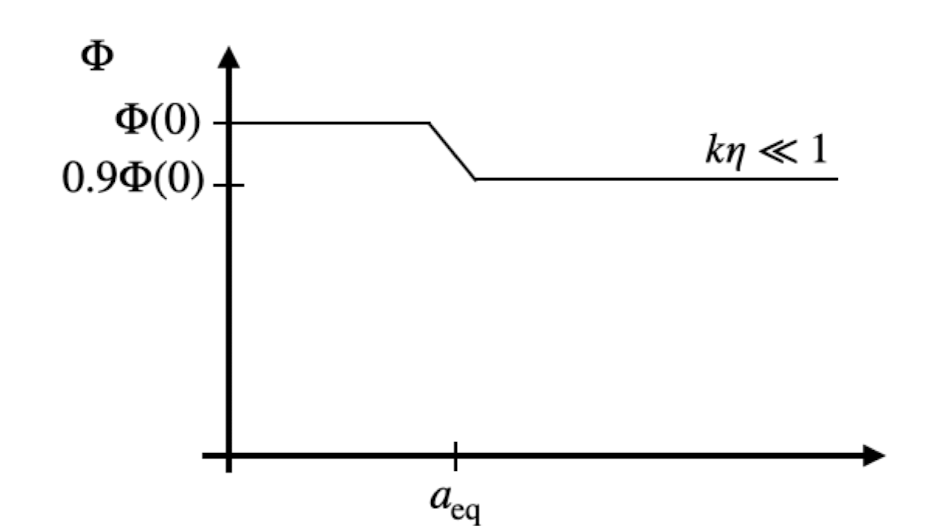
\includegraphics[scale=0.4]{Figures/finn.png}
        \end{center}
        \caption{The potential on large scales as the Unvierse
          traverses matter-radiation equality.}
        \label{fig:}
        \end{figure}
        
        \subsubsection{Horizon crossing $ k \eta \sim 1 $}%
          \label{sub:ketasim1}
          
          For this limit, if \( k \eta \sim 1  \), then 
          \begin{align}
            \label{horzing crossing = 1}
            a_{H} \sim 0.03 \gg a_{eq}.
          \end{align}

          Now, under this assumption, i.e. \( a_{H} \gg a_{eq} \),
          we can drop the photon terms as the modes of interest
          enter the horizon during matter domination. After
          resorting to the Einstein's equation and the previous
          systems of Fourier equations (\ref{all CMB equations}),
          we will eventually obtain 
          \begin{align}
            \label{horizon crossing ~ 1 equation}
            \bigg[\frac{2k^2}{3 a^2 H^2} + 3 \bigg]
            \tilde{\Phi}^{\prime} + \bigg[k^2 + \frac{9a^2
            H^2}{2}\bigg]
           \bigg(\frac{i \tilde{v}}{k} + \frac{2
          \tilde{\Phi}}{3 a H} \bigg) = 0 
          \end{align}
    
          If we differentiate this once more and we will find that
          \( \tilde{\Phi} \) is actually constant, which means the
          growth function \( T(k) \approx 1 \implies
          \Phi(\textbf{k, a}) \approx \Phi_{p}(\textbf{k}) D_1 (a)
          \).

          \begin{figure}[h!]
          \begin{center}
            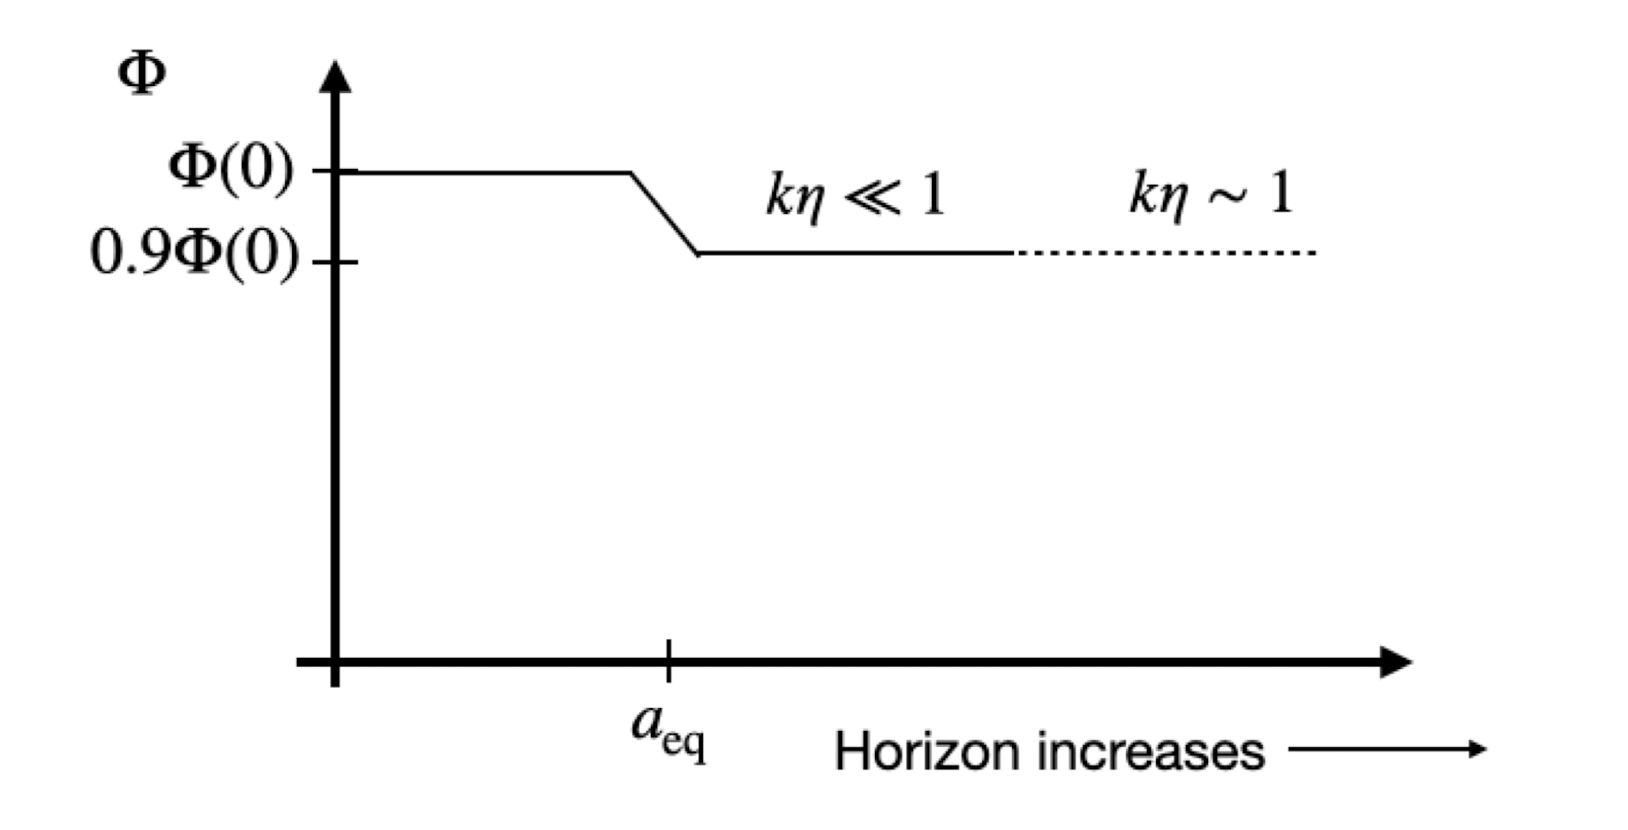
\includegraphics[scale=0.4]{Figures/finn2.png}
          \end{center}
          \caption{As modes enter the horizon during matter
            domination, the potential remains constant.}
          \label{fig:finn2}
          \end{figure}
         
         \subsection{Perturbation on small scales}%
          \label{sub:Perturbation on small scales}
          Now for small scale modes, we are essentially describing
          them during radiation domination (that's where they
          first enter), and thus we only need to consider the
          radiation terms in the Boltzmann system, as the matter
          terms are suppressed by a factor \( \rho_{dm} / \rho_r
          \). Again to solve this, we use (i) one of Einstein's
          equations, (ii) \( H^2 = 8 \pi G \rho_r /3 \), (iii) \(
          \eta \approx (aH)^{-1}\) during radiation era, (iv) and
          lots of good luck. 

          We then get the differential equation, 
          \begin{align}
            \label{small scales equation}
              \tilde{\Phi}^{\prime \prime} + \frac{4}{\eta}
              \tilde{\Phi}^{\prime} + \frac{k^2}{3} \tilde{\Phi}
              &= 0.
          \end{align}
          The analytic solution to this is given by 
          \begin{align}
            \label{analytic to small scales evolution}
            \tilde{\Phi} &= 3 \tilde{\Phi}_{p}
            \bigg[\frac{\mathrm{sin}(k \eta / \sqrt{3} ) - (k
            \eta / \sqrt{3} ) \mathrm{cos}(k \eta / \sqrt{3} )  }{
            (k \eta / \sqrt{3} )^3} \bigg].
          \end{align} The implication here is that they enter the
          horizon during radiation era and then decay and
          oscillate. 
          \subsection{Matter density perturbation}%
            \label{sub:Matter density perturbation}
            We can do the similar procedure (but harder) for the
            matter density perturbation \( \tilde{\delta} \) as
            well, which they are of the form 
            \begin{align}
              \label{matter density pert solution}
              \tilde{\delta}(k, \eta) \approx 9.6 \Phi_{p}
              \mathrm{ln}(0.44 k \eta).
            \end{align} The upshot here is that they enter the
            horizon during the radiation and grow logarithmically.
            Though to obtain a more accurate result, we have to
            also consider the fact that at later times matter
            grows and it will get coupled to the potential, i.e.
            in the limit \( \rho_{dm} \tilde{\delta} > \rho_{r}
            \tilde{\Theta}_{r, 0} \). 

            With this consideration, we need to write the
            Boltzmann system in terms of new variable y and
            consider the no anisotropic stress assumption, 
            \begin{align}
              \label{new variable y and no anisotropic stress}
              \frac{\mathrm{d}\tilde{\delta}}{\mathrm{d}} +
              \frac{i k v}{a H y} &=  - 3
              \frac{\mathrm{d}\tilde{\Phi}}{\mathrm{d}} \\ 
              \frac{\mathrm{d}\tilde{v}}{\mathrm{d}y} +
              \frac{\tilde{v}}{y} &= \frac{ik \tilde{\Phi}}{a H
              y}, 
            \end{align} where \(  y = a / a_{eq} \).

            Again we adopt the
            Einstein's version of the Poisson equation that links
            the density and potential: 
            \begin{align}
              \label{einsten version of poisson for density and
              potential}
              k^2 \tilde{\Phi} &=  \frac{3y}{2(y+1)} a^2 H^2
              \tilde{\delta}. 
            \end{align}

            

            Finally if we solve them all, we will obtain that \(
             \tilde{\delta} \propto D_1(y) \approx y \).
             So the two solutions becomes 
             \begin{align}
              \label{D_1 of matter}
               D_1(y) &=  y + \frac{2}{3}. 
             \end{align} 

             Note that we will also get second
             solution for \( \tilde{\delta} \) as well, but it
             goes as \( D_2(y) \propto y^{-3/2}  \) and thus
             unphysical.

             Explicitly, \( D_2(y) \) goes like 
             \begin{align}
               \label{D_2(y) of matter}
               D_2(y) &= D_1(y) \mathrm{ln} \bigg[
               \frac{\sqrt{1+y} + 1}{ \sqrt{1+y} - 1 }  \bigg] -
               2 \sqrt{1+y} 
             \end{align}

            \subsection{The matching era and the transfer
            function}%
              \label{sub:The matching era and the transfer
                        function}
              It is possible to match the two solutions of \(
              \tilde{\delta}   \),
              \begin{align}
                \label{matching Ds}
                A \tilde{\Phi}_{p} \mathrm{ln} ( \frac{B
                y_{m}}{y_H} ) &= C_1 D_1^{\prime}(y_{m}) + C_2
                D_2^{\prime}(y_{m}) \\ 
                A \frac{\tilde{\Phi}_{p}}{y_m} &= C_1 D_1^{\prime}(y_{m}) + C_2
                D_2^{\prime}(y_{m}) 
              \end{align}
              By doing so and solve for the constants, we will get a
              factor an extra factor for \( \tilde{\delta} \),
              which is the transfer function
              \begin{align}
                \label{transfer function for matter}
                T(k) &=  \frac{12 k_{eq}^{2}}{k^2} \mathrm{ln}
                \bigg[\frac{k}{8 k_{eq}} \bigg].
              \end{align}

              \subsection{Growth function at late times}%
                \label{sub:Growth function at late times}
                  To solve for the growth function at later
                  times, we can use the following equation 

                  \begin{align}
                    \label{growth function at late times}
                    D_1(a) &= \frac{5 \Omega_{m,0}}{2}
                    \frac{H(a)}{H_0} \int_{0}^{a}
                    \frac{\dd[]{a^{\prime}}}{(a^{\prime}H(a^{\prime})/H_0)^3} 
                  \end{align}

              \subsection{Evolution of the matter power
              spectrum}%
                \label{sub:Evolution of the matter power
                            spectrum}
                Now we can write down single-handedly one of the
                most important quantity in cosmology - the
                (matter) power spectrum 
                \begin{align}
                  \label{matter power spectrum}
                  P_{\delta}(k, a) &= 2 \pi^2 \delta_{H}
                  \frac{k^n}{H_{0}^{n+3}} T^{2}(k)
                  \bigg(\frac{D_1(a)}{D_1(a=1)} \bigg)^{2}.
                \end{align} Here \( \delta_H \) is some
                normalization constant. 

                \subsection{Numerical approaches}%
                  \label{sub:Numerical approaches}
                  
                  There are a group of physicists primarily
                working on simulating all these perturbations,
                and generally there are several assumptions made
                for most simulations due to technical limitations
                and limitations in numerical mathematics. 

                \subsubsection{Matter-only}%
                  \label{sub:Matter-only}
                  We can safely ignore dark energy in our
                  simulation since it does not have any spatial
                  fluctuations but contributes only to the
                  background expansion. This background expansion
                  can be taken off by simply re-scaling the
                  physical coordinates of the particles to
                  comoving coordinates. 

                \subsubsection{Use of Newtonian physics}%
                  \label{sub:Use of Newtonian physics}
                  If the simulation "box" is not too big, and
                  gravity is not too strong anywhere, then one
                  can use Newtonian physics for the evolution. By
                  too big, it means that the size of simulation
                 contains non-uniform density distribution to the
                 point where Newtonian limit (linear-limit) fails
                 to approximate the result. And by too strong it
                 means, quantities like black holes. 

                \subsubsection{No formation of galaxies}%
                  \label{sub:No formation of galaxies}
                  The main interests here is the matter spectrum,
                  whereas galaxies are form at late stages. 

                  Although, they induces \( < 15
                  \percent \) corrections to the power spectrum
                  at nonlinear scales, which is still significant
                  and it is a topic of current investigation.

      \section{CMB}%
        \label{sec:CMB}
        In this section, we will delve into the physics and
        mathematical construction behind the CMB. 

        \subsection{Blackbody Law}%
          \label{sub:Blackbody Law}
          First, we can use the \textit{blackbody law} to obtain a
          rough estimate on the CMB temperature. To do so, we
          introduce first the solid angle \( B_{\lambda} (T)
          \dd[]{\lambda} \dd[]{A} \mathrm{cos}(\theta)
          \dd[]{\Omega} \), with 
          \begin{align}
            \label{planck temperature distribution}
            B_{\lambda}(T) &= \frac{2h c^2 /
            \lambda^5}{e^{hc/ \lambda k T} - 1 } \\ 
            \label{planck temperature distribution in frequency} 
            B_{\nu}(T) &= \frac{2h \nu^3 /
            c^2}{e^{h\nu/ k T} - 1 }.
          \end{align}
          By \textbf{Wien's law},

          \begin{align}
            \label{wien's law}
            \lambda_{\mathrm{max}} T &= 0.0029 \mathrm{mK}, 
          \end{align} we can then estimate that CMB is \( 2.1
          \mathrm{K} \).


      \begin{figure}[h!]
      \begin{center}
        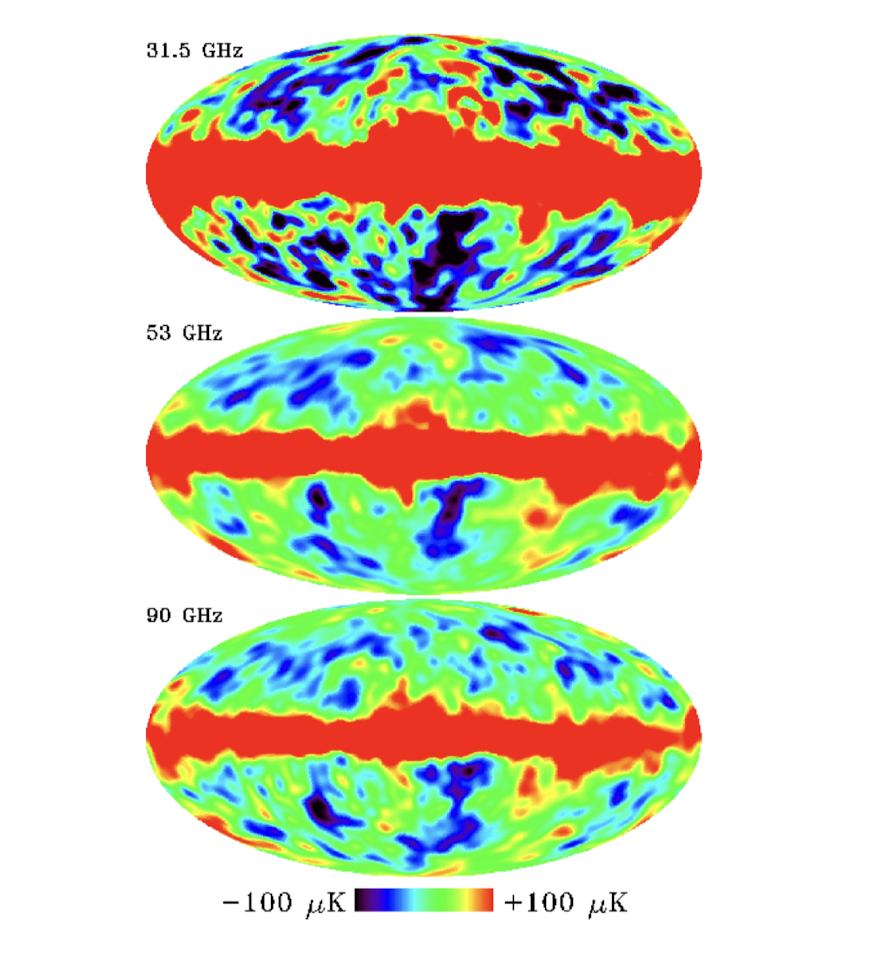
\includegraphics[scale=0.5]{Figures/cobecmb.png}
      \end{center}
      \caption{Temperature fluctuations in the microwave
        background (with respect to the mean) at different
        frequencies, as measured by COBE. The red area
        corresponds to emission from our own Galactic plane.}
      \label{fig:cobecmb}
      \end{figure}
      

      \textbf{\underline{Comments:}} Whatever, just skip this\ldots


      \subsection{Angular decomposition of CMB}%
        \label{sub:Angular decomposition of CMB}
        We can begin by defining the temperature perturbation as 
        \begin{align}
          \label{temperature peturbations}
          \Theta(\textbf{x}, \hat{\textbf{p}}, \eta) &=
          \frac{T(\textbf{x}, \hat{\textbf{p}}, \eta) -
          \bar{T}(\eta)}{\bar{T}(\eta)},
        \end{align} and decompose this with the spherical
        harmonics so that 

        \begin{align}
          \label{temperature perturbations in spherical harmonics}
          \Theta(\textbf{x}, \hat{p}, \eta) &=
          \sum_{l=0}^{\infty} \sum_{m = -l}^{l} a_{lm} (
          \textbf{x}, \eta   ) Y_{lm}( \hat{\textbf{p}} )
        \end{align}

        It is also necessary to Fourier transform over the
        perturbation as 
        \begin{align}
          \label{fourier-transformed temperature field}
            \Theta(\textbf{x}, \hat{\textbf{p}}, \eta) &= \int
            \frac{\mathrm{d}^{3} \textbf{k}}{(2 \pi)^{3}}
            \tilde{\Theta}(\textbf{k}, \hat{\textbf{p}}, \eta)
            e^{i \textbf{k} \cdot \textbf{x}},
        \end{align} we do so because we can spread the CMB into
        different modes for study. 

        \textbf{\underline{Remarks: }} Note that \( \eta = \eta_0
        \) since this is as far as we can probe. Yes life is
        short, although there are goals to compare CMB at
        different \( \eta \), which will be a century project.

        \subsection{connection to Boltzmann theory}%
          \label{sub:connection to Boltzmann theory}
          To resonate with previous section's results, we have
          that, before recombination \( \Theta = (\Theta_0,
          \Theta_1) \). And after recombination 

          \begin{align}
            \label{after recombination to CMB}
            \frac{1}{(-1)^{l}} \int_{-1}^{1} \dd[]{\mu} P_{l}(H)
            \Theta( \textbf{x}, \hat{\textbf{p}}, \eta )
          \end{align}


\section{Brief History of the Universe again}%
  \label{sec:Brief History of the Universe again}

\subsection{Relevant scales}%
  \label{sub:Relevant scales}
  
  We define the reduced Planck mass as \( M_p = \sqrt{ \bar{h} c / 8 \pi G }
  \approx 2.4 \times 10^{18} \mathrm{GeV/c^2} \), and we adopt the natural
  unit. 
  Note that the inflation ends at \( H_I \sim \sqrt{ \bar{h} \rho / 3 c
  M_{p}^{2}}  \approx 10^{13} \mathrm{GeV / \bar{h}} \)


  \subsection{slow roll parameter}%
    \label{sub:{slow roll parameter}
    
  The time of the universe is given by the rest frame of the CMB photon, i.e. the pull back \( u|^{\mu} \).

  We also define the principal slow roll parameter as \( \epsilon  =
  - \dot{H}/H\).

  \begin{figure}[h!]
  \begin{center}
    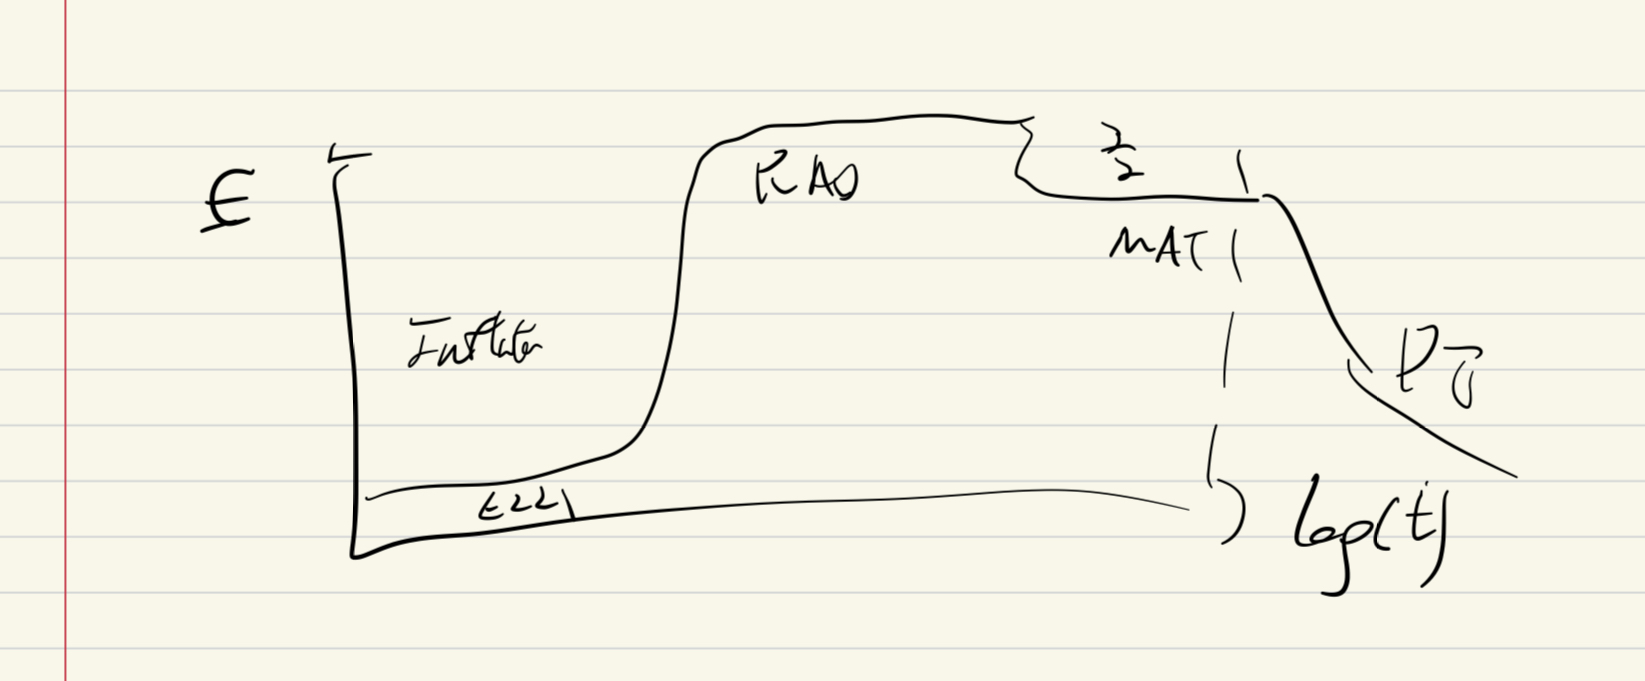
\includegraphics[scale=0.2]{Figures/slowrollgraph.jpeg}
  \end{center}
  \caption{slow roll across Universe time, note that there is no evidence
    during the $ \epsilon \ll 1 $ regime.}
  \label{fig:slowrollgraph}
  \end{figure}
  

  \begin{figure}[h!]
  \begin{center}
    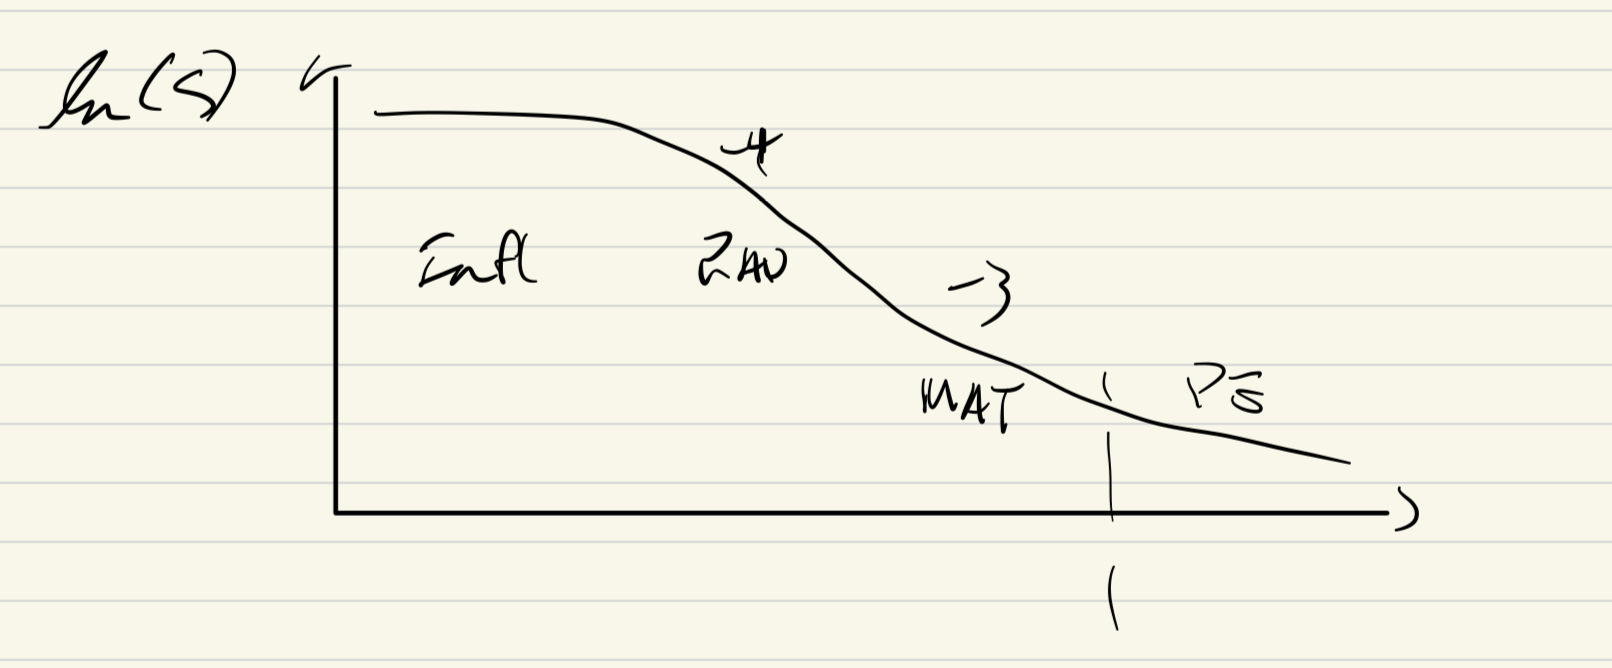
\includegraphics[scale=0.2]{Figures/lnslowrollgraph.jpeg}
  \end{center}
  \caption{logarithm of slow roll across Universe time.}
  \label{fig:lnslowrollgraph}
  \end{figure}
  
Note the from the Friedmann equation, we can find for the relation of
scale factor with respect to \( \rho \) along the state parameter \(
\omega\), then we should get 
\begin{align}
  \label{slow roll parameter}
  \epsilon = \frac{3}{2} (1 + \omega),
\end{align} and from theory, we get that the inflation happens at $
10^{-35}s $. 
\vspace{0.5cm}

Typically, 

\begin{align}
  \label{slow roll scenarios}
  \begin{cases} 
    \mathrm{Inflation: } 0 < \epsilon \ll 1; \hspace{0.5cm}
    \frac{\dot{\epsilon}}{\epsilon} \ll H \\ 
    \mathrm{Radiation: } \epsilon \approx 2, \textnormal{the
    transition to the second is 100000 yrs roughly} \\ 
    \textnormal{Matter}: \epsilon \approx  \frac{3}{2} \\ 
    \textnormal{Dark Energy}: \epsilon \approx 0.6 (\mathrm{today})
  \end{cases}
\end{align}


\subsection{perfect fluid and driving mechanics}%
  \label{sub:perfect fluid}
  
  Here as usual, we take the perfect fluid assumption, then we shall get
  under the assumption 
  \begin{align}
    \label{fluid assumption}
    \epsilon = \frac{3}{2} (1 + \omega) \approx 0 \implies \oemga
    \less -1; \hspace{0.5cm} H(t) \approx H_0 a^{- \epsilon(t)} 
  \end{align}

Now we are in the position to ask what drive inflation, 

If we first assume this is fundamental; \( \phi(t) = \langle \hat{\Phi}(x)
\rangle   \). 

We can also define the fluctuation in energy-momentum tensor 
\begin{align}
  \label{fluct energy tensor}
  \langle \hat{T}_{\mu \nu}^{\phi} \rangle  = \langle
  \partial_{\mu}^{} \hat{\phi} \partial_{\nu}^{} \hat{\phi} \rangle + g_{\mu
  \nu} \langle  \mathcal{L}(\hat{\phi}) \rangle (t), 
\end{align} note that this is a very non-trivial step but generally on
a typical homogenous inflation setting, we can always guarantee to find a
FFF such that the fluctutation of fields are well-defined.
 

 We now define the energy density and pressure as 
 \begin{align}
  \label{inflaton pressure and energy density}
   P &= \frac{\dot{\phi}^{2} }{2} - v(\phi) \\ 
    \rho &= \frac{\dot{\phi}^2}{2} + V(\phi), 
 \end{align}
And the slow roll parameter becomes 
\begin{align}
  \label{slow roll becomes}
  \omega = \frac{P}{\rho} = \frac{\dot{\phi}^2}{2} - V(\phi) /
  \frac{\dot{\phi}^2}{2} + V(\phi) \sim -1
\end{align} 

 Now, one potential way to produce inflation is perhaps the expectation
 of the certain quantites like, \( \hat{F}_{\mu \nu} \hat{F}^{\mu
 \nu} \), i.e. higher-spin fields, can drive the inflation if we pick a
 potential such that it exhibits Higgs-like potential, and with the field
 starting at the unstable equilibrium.

* \underline{How inflation ends?} 

The short answer is that we do not know still, as there is no observation
at the end of inflation.


\subsection{Quick review of thermodynamics}%
  \label{sub:Quick review of thermodynamics}

  In inflation, we assume istropic, thus \( \dd[]{S} = 0 \). We also define
  \( U = \rho V \), then we get 
  \begin{align}
    \label{1st law of TD in inflation}
    \dd[]{U} = \dd[]{(\rho V)} = V \dd[]{\rho} + \rho \dd[]{V}.
  \end{align} We can see that with this law, then \( \rho \dd[]{V}
  \approx - P \dd[]{V} \implies W > 0, \mathrm{ if } P < 0; \rho \approx
  \mathrm{const.} \) Now, the big question is where does this energy
  comes from when as the Universe expands. 

  \subsubsection{Energy comes from gravity}%
    \label{sub:{Energy comes from gravity}



   \begin{align}
    \label{energy comes from gravity}
     - \frac{3 H^2}{8 \pi G} + \rho \equiv 0, \hspace{0.5cm}( 00
     - \textnormal{component of EFE} )
   \end{align} 


\subsection{perturbative methods}%
  \label{sub:perturbative methods}
  

 \begin{align}
  \label{interaction field}
  \mathcal{L}_{\mathrm{int}} &=  - y \phi \bar{\psi} \psi - \frac{g}{2}
   \phi^2 \chi^2,   
 \end{align} where all the fields here are the standard model fields,
 with \( \phi \) being the inflaton. 

There are two ways to go about studying the interaction, for the Yukawa term,
we can do perturbative QFT, which we get the tree-level decay rates as 

\begin{align}
  \label{yukawa tree-level decay}
  \Gamma_{\phi \to \bar{\psi} \psi} = \frac{|y|^2}{4 \pi} E_{\phi},
\end{align} where \( E_{\phi} = \sqrt{p_{\phi}^{2} + m^2} \approx  \),
and 
\begin{align}
  \label{yukawa tree-level decay 2}
  \Gamma_{\phi \to \chi \chi} = \frac{|g|^2}{4 \pi}
  \frac{|\phi_0|^2}{E_{\phi}}, 
\end{align} 
\underline{\textbf{Remarks: }} Please note that although the yukawa is 4
fields interaction, but however under the condensate assumption for the
inflaton, we can write it as \( \phi = \phi_0 + \delta \phi \), thus we get
the resulting 3 scattering diagram, the dashed lines refers to \( \delta
\phi \) as always. 


\subsection{Non-perturbative methods}%
  \label{sub:Non-perturbative methods}
  
  In the non-perturbative QFT analysis, one may use the technique
  of parametric resonance.  

  Say given the inflaton oscillating in the well potential, with the
  equation of motion as 
  \begin{align}
    \label{eom of inflaton field oscillating in the potential}
    ( \partial_{t}^{2} + 3 H \partial_{t}^{} + m_{p}^{2} )
    \phi_{0}(t) &= 0 \\ 
    ( \partial_{t}^{2} + m_{p}^{2} - \frac{3}{2} \dot{H} -
    \frac{g}{2} H^2 ) ( a^{3/2} \phi_0  )  = 0
  \end{align}

  At the end, we will obtain the Mathiew equation for the equation of
  motion with parametric resonance. And note that the eom has a form 
  \begin{align}
    \label{Mathieu equation}
    \ddot{x} + ( a + 2b \mathrm{cos}(t)  ) x = 0
  \end{align}

  And in the a = 2b regime, we recover the typical simple harmonic
  oscillator. 








\bibliographystyle{unsrt}
\bibliography{references.bib}
        
\end{document}
